\selectlanguage{english}
%%%%%%%%%%% Capitulo 2 Metodologia %%%%%%%%%%%%%%%%%%%%%%%%%%%%%%%%%%%%%%%%%%%%%%%%%%%%%%%
%\setcounter{chapter}{1}
\chapter[Methods]{Methods}\label{c2:Methods}
In this chapter we shall outline the methods used in the set of studies that form the thesis. 
Generic 
molecular dynamics and quantum chemistry methods are not included for the sake of succinctness. 
We focus on the contents that cannot be found in textbooks since they are either recent or 
rather specific to the contents of this thesis. In any case, I would like to give credit to 
the authors who have published those textbooks and leave them as reference for anyone seeking 
a fundamental training. A straightforward approach to statistical computer simulations can be 
achieved through the classic textbook of 
Frenkel\cite{frenkel2001understanding} in addition to more unknown and modern books like 
those of Shclick\cite{Shclick2013}, Smith\cite{Smith2014} or 
Berendsen\cite{HermanJ.C.Berendsen2007_v2}. To study Quantum Chemistry, the 
classic text of 
Zsabo and Osmund\cite{szabo2012modern} must be cited in addition to the more modern book of 
Cramer\cite{Cramer2004_v2}. In order to get insight into classical mechanics and statistical 
mechanics, the works of Marion\cite{Jefferys1966}, Goldstein\cite{Goldstein}, 
Tuckerman\cite{tuckerman2010statistical} and McQuarrie\cite{mcquarrie1973statistical} must be cited.

%%%%%%%%%%%%%%%%%%%%%%%%%%%%%%%%%%%%%%%%%%%%%%%%%%%%%%%%%%%%%%%%%%%%%%%%%%%%%%%%%%%%%%%%%%%%
\section{Molecular Simulation}\label{sec:molecularsimulation}
%%%%%%%%%%%%%%%%%%%%%%%%%%%%%%%%%%%%%%%%%%%%%%%%%%%%%%%%%%%%%%%%%%%%%%%%%%%%%%%%%%%%%%%%%%%%
The coming of the digital age in the eighties up to the present produced 
groundbreaking transformations to most aspect of human life: culture, economics, 
communication, politics... Science would not be different. 

Before the widespread of computation, Science was a 
symbiotic organism formed by two 
individuals: experiment and theory in the pen and paper sense. Both parts communicated and 
reinforced each other in the development of the fields. With the exponential growth in 
computer power a third term was added to the equation: simulation. 

Modelling has always been key in Science. This involves proposing a simplified image of the system 
and the equations that govern its behavior. After this, experimentalists would 
use the model to fit their data and theoreticians would solve the equations analytically. 
Unfortunately, this normally involves using very simple systems or doing big mathematical 
assumptions. With modern computers, for the first time, scientists were able to numerically solve 
the equations proposed by theoreticians in 
order to obtain detailed pictures of complex model systems. These simulations give 
interpretation to experiment and a predictive guide for experimentalists. 

In the case of molecular simulation, a chemical system is modeled as a collection of particles 
which sample phase space following the evolution of a model hamiltonian. Once the sampling is 
finished Statistical Mechanics is applied to obtain observables that can be compared to 
experiment or serve to predict or interpret it. The recipe for a molecular simulation always 
involves three main ingredients: 

The first ingredient is the Chemistry that we are studying and how we plan to 
represent it on the 
computer. For this we must choose the composition of the system and its size such that it is as 
representative of the real system as possible. In this thesis we simulated, among others, the 
actinyl hydrated ions in the solution with 1500 water molecules and inside montmorillonite clay. 
These systems will represent a uranyl cation at infinite dilution and a true montmorillonite 
infinite crystal containing uranyl cations in its interlayer. 

The second ingredient is the model hamiltonian of the system. This hamiltonian will give the 
approximate energy of the system as a function of particle positions and velocities. If the 
system is small and/or the evaluation of forces and energies has to be done few times, the 
hamiltonian can be the quantum mechanical (\gls{qm}) hamiltonian. On the contrary, if the system is 
large and/or many energy or force evaluations are necessary, a classical hamiltonian in the form of 
a 
force field or interaction potential must be used. In a force field the energy is given as a
simple analytic function of particle coordinates (charges, bonding tensions, bending tensions, 
dihedrals ...) which is parametrized to reproduce experimental data (empirical force fields) or 
QM data (ab initio force fields) or both. If the system is very large but  
QM effects are explicitly needed, such as if chemical reactions or light 
absorption take place, a hybrid method must be used. These methods are known as QM/MM 
approaches and 
are based on treating a small but important part of the system quantum-mechanically and the rest 
using a classical force field. In this work we shall consider mostly ab initio force fields 
developed specifically for the systems under study. In this way we were able to work with 
larger 
systems keeping a near QM-level description at force field cost.

The third ingredient is the phase-space sampling method. The particles that constitute matter 
are 
in constant motion going from one position and velocity state to another. This continuum of 
states (in classical terms) is what is known as phase-space. The phase-space of most non-trivial 
chemical systems is too large to be studied exhaustively. Fortunately, only a limited part of 
this space is significant as most of these states are highly unlikely and statistically 
irrelevant. Therefore, we can resort to sampling only relevant areas of phase space. If the 
dynamics of the system are not of interest, the configuration-space rather than the phase space can 
be sampled.\newline Configuration-space is the space of all possible particle positions. Some 
techniques 
that sample configuration-space are geometry optimization and Monte Carlo simulations.

\begin{figure}
\centering
         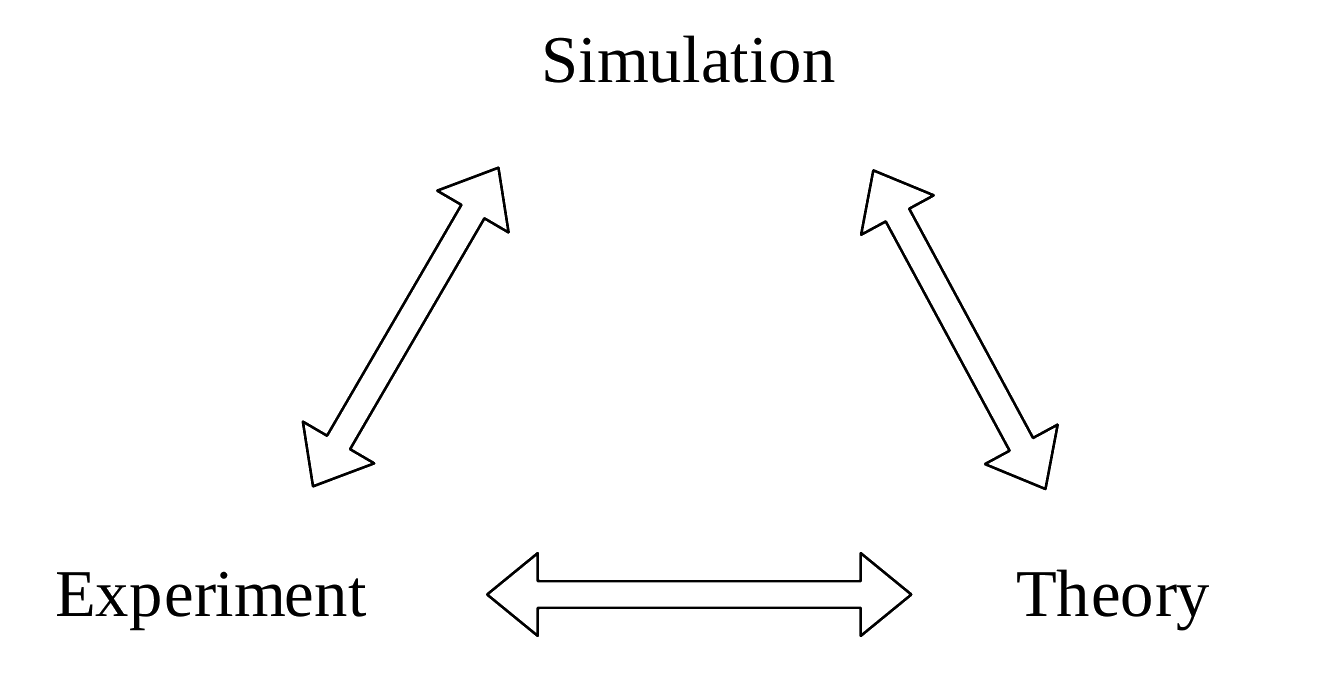
\includegraphics[width=0.7\textwidth]{images/ResearchTriangle.png}
        \caption[Research Triangle]{The research 
triangle showing the synergy between theory, experiment and simulation.}
        \label{fig:1}
\end{figure}

The least expensive method is geometry optimization in which the energies and geometries of the 
system energy minima or saddle points are obtained by an optimization procedure. This method 
has the limitations of only sampling states close to the initial configuration, which can be 
troublesome in complex potential energy surfaces, and it models entropic and solvent effects 
in a crude fashion\cite{Cramer2004_v2}. In contrast,  Monte Carlo or Molecular Dynamics 
(\gls{md})
methods do Boltzmann sampling of -ideally- the full configuration or phase space and includes 
solvent and 
entropic effects explicitly. Monte Carlo simulations sample stochastically configuration space 
by making random moves in the system and accepting them into the statistics with a probability 
based on their Boltzmann weight\cite{frenkel2001understanding}. MD is based on 
the propagation of the equations of motion of the system and the resulting trajectory is 
analyzed. MD is theoretically founded on the ergodic hypothesis which states 
that ensemble average properties are equal to time averages properties if the phase space is 
sampled fully.\cite{Smith2014} In many cases this hypothesis is a reasonable assumption, but in 
cases with high free energy barriers between relevant states the trajectory might 
be stuck in one of the states and not sample the other. To have access to these states within 
the MD simulation approach, enhanced sampling methods like 
metadynamics (\gls{metad})\cite{Valsson2016,bussi2015free} can be used. In enhanced sampling 
methods 
a bias potential is added to the simulation hamiltonian in order to force sampling in the 
relevant states of the system. The extra complexity of enhanced sampling simulations is 
rewarded with the generation of a free energy surface of the system. Finally, in order to 
calculate the free energy difference between different chemical systems free energy 
perturbation methods can be used\cite{Shirts2013_v2}. 





\section{Metal Ion Force Fields}\label{sec:MIFF}

Ions in solution are among the first systems to be studied with MD. 
The reason being that there is no question about their importance. They 
are present in all natural waters, in an enormous part of industrial processes, and are crucial to 
biochemistry (one third of pdb protein structures contain metal ions\cite{solomon1996volume}).

The first simulation of ions in water was performed by Heinzinger and Vogel over 50 years 
ago studying aqueous LiCl\cite{heinzinger1974molecular}. They modeled water with the ST2 model of 
Rahman and Stillinger\cite{rahman1971molecular} and obtaining van der Waals parameters for the 
ions from their iso-electronic noble gas parameters of 
Hogervost\cite{hogervorst1971transport}. Despite the simulation capabilities of the time, the 
simulations showed good agreement between the first-shell properties and X-Ray diffraction 
experimental data. Furthermore, they predicted the faster rotation time of the 
first-shell water molecules with respect to bulk in agreement with \gls{nmr} data. Other 
pioneers 
and 
front-runners in this research were Jorgensen et 
al.\cite{jorgensen1982quantum,chandrasekhar1984energy,jorgensen1983comparison}
and $\AA{}$qvist\cite{aqvist1990ion}  in the eighties and nineties respectively.  

The most common feature across popular aqueous ion force fields is their functional 
form:

\begin{equation}\label{eqLJ}
E_\text{int}=
\sum_{i=1}^N\sum_{j>i}^N 
\frac{q_iq_j}{4\pi\epsilon_0 r_{ij}}+ 
\sum_{i=1}^N\sum_{j>i}^N
4\epsilon_{ij}\left[\left(\frac{\sigma_{ij}}{r_{ij}}\right)^{12}-\left(\frac{\sigma_{ij}}{r_{ij}}
\right)^6\right]
\end{equation}

Where $E_\text{int}$ is the interaction energy between all the particle pairs $i j$. We shall 
not 
discuss the water force field which has been reviewed 
elsewhere\cite{PhysChemChemPhys_Vega_2011}. Many other functional forms exist: 
Born-Mayer, Mie, Morse etc.\cite{Li2017} Nevertheless, the one presented above is the most 
representative in the literature.  

The first term of the equation is the electrostatic term which features the integer charge 
of the ion and the partial charges of the water model. This term is generally evaluated using an 
Ewald sum variant\cite{frenkel2001understanding}. We neglect two effects in this force field 
approach: charge transfer to the 
first shell and polarization of the water molecules. They 
cannot be represented explicitly within the pair interaction approximation: all forces depend 
on the atom pair relative positions. This makes the force calculation algorithm 
computationally fast. Charge transfer and polarization are intrinsically many-body effects and 
not pair interaction effects. Modelling charge transfer and polarization in pair 
potentials remains one of the key parts of ion interaction potential development. Force fields 
which include many-body effects in pair potentials are know as \textit{effective pair potentials}.

The second summation of Equation \ref{eqLJ} is the van der Waals interaction between 
the atom pairs. In ion-water interactions they are less important in magnitude than 
electrostatics but crucial to the modelling. In Equation \ref{eqLJ} this molecular interaction 
is described by the Lennard-Jones function.



Lennard-Jones based force fields have proven to be fairly robust in treating monovalent ions 
in a simple and inexpensive fashion. But, their performance degrades heavily on multiply-charged 
cations or molecular cations\cite{Li2017,Li2015,Li2013}. This is a consequence of 
the increasing weight of charge transfer and polarization as the cation charge increases. This 
is the Achilles' heal of Lennard-Jones potentials.


Regardless of its functional form, the parameters of the force field are fit with respect to 
experimental data (empirical force fields) and/or \textit{ab initio} calculations (\textit{ab 
initio} force fields). In cation force fields the $q_i$ are 
given by the water model and the charge of the ion in particular. Only the Lennard-Jones 
parameters remain to be fit. 

If the fitting is done with respect to empirical data, the force field guarantees that 
properties introduced in fitting data set are reproduced. It is reasonable to expect that 
properties that correlate with the fit data are fairly well reproduced too. Free energy of 
hydration and ion first-shell distance are an example of this\cite{Li2015}. Further 
extrapolation should be done with additional skepticism. 

\begin{figure}
     \centering
         \includegraphics[width=\textwidth]{images/E_int.png} 
        \caption[Many body effects in the Po(VI) hydrate.]{QM interaction energies of 
\ce{[Po(H2O)_n]^{4+}(g)} per water molecule as a function of n at the MP2 level of 
theory.\cite{Ayala2008} This example illustrates how the interaction energy of a highly charged 
cation with its first shell water molecules is a many-body interaction. If this was not the case, 
a horizontal line would be obtained.}
        \label{PoEint}
\end{figure}

\textit{Ab initio} force fields are parametrized with respect to energies and molecular 
structures obtained from quantum chemistry calculations. This strategy has several advantages. 
If the sampling of the system potential energy surface is exhaustive enough and at a 
reasonable level of theory, the prediction of information for which the force field was not 
specifically designed is 
typically better than using empirical force fields. In addition, the fitting data sets can be 
generated easily. Especially since medium-level calculations produce satisfactory results in 
most properties. This is particularly appreciated in experimentally challenging 
systems like radioactive elements. \textit{Ab initio} force fields have a clear improvement 
path; just add more structures or improve the level of theory. For these reasons the 
interaction potentials developed in this thesis will all be classical force fields based on 
\textit{ab initio} calculations.

The traditional strategy to obtain the QM data is to calculate the 
interaction energies of the monohydrate, \ce{M^{+n}}-\ce{H2O}, at different metal oxygen 
distances. This has two shortcomings for highly charged cations. 

\begin{figure}
     \centering
         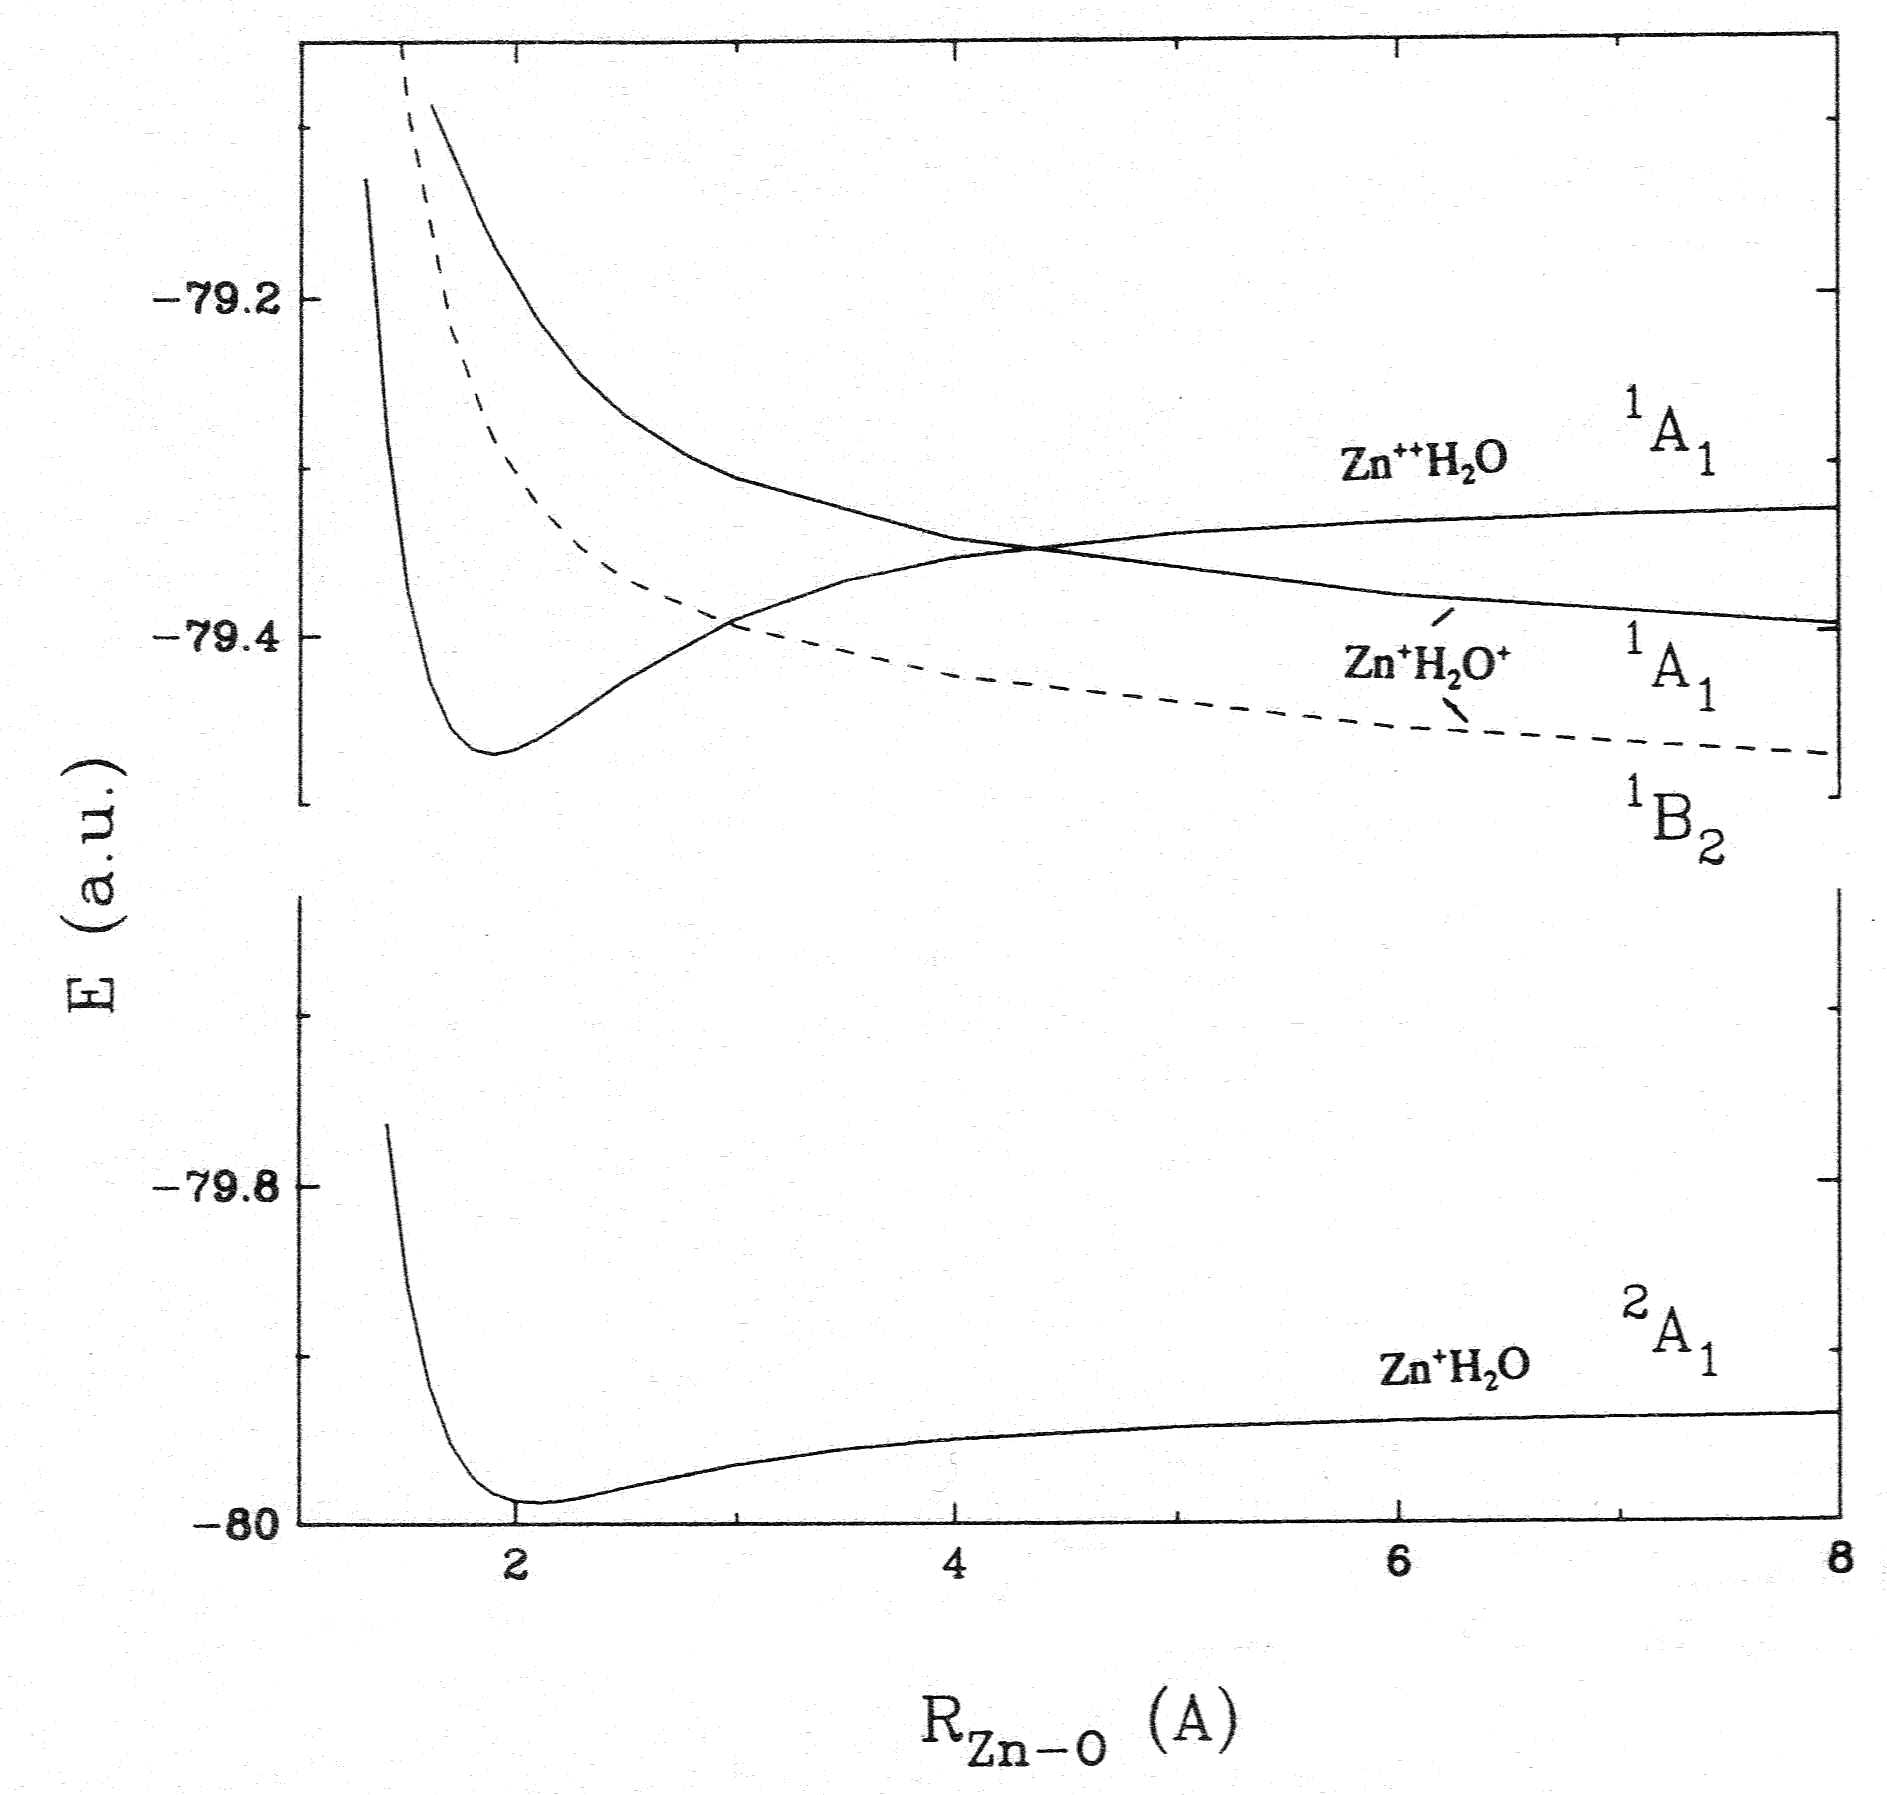
\includegraphics[width=0.7\textwidth]{images/ZnQM} 
        \caption[Charge transfer in \ce{[Zn*(H2O)]^{2+}}]{Hartree Fock energies for the ground 
state 
of  \ce{[Zn*(H2O)]^{+}} ($^2A_1$) and 
\ce{[Zn*(H2O)]^{2+}]} lowest states ($^1A_1$ and $^1B_2$). For the monovalent there are no low 
lying excited states but for the divalent there are two charge transfer states which are the lowest 
in energy at long distances. Reproduced with permission of the 
authors\cite{JPhysChem_ESM_1992}.}
        \label{ZnQM}
\end{figure}

The first is that the average total hydration enthalpy is highly overestimated. The cause of 
this is that the interaction energy in the monohydrate is much more 
negative than the interaction energy of the individual water molecules around an ion when 
fully solvated. In other words, the interaction energy of the metal with its first shell 
is different from the interaction energy of the monohydrate times the coordination number. 
This is because when going from the monohydrate to the n-hydrate the polarizing 
capability per water molecule of the ion decreases with n. The 
interaction energy per water molecule decreases as you increase the number of molecules in the 
first shell as is illustrated in Figure \ref{PoEint}. This means that the interaction energy of 
a cation with its 
first shell is a many-body case (in this case a ``body'' refers to a water molecule). In 
addition, 
the water-water repulsion in the fully-hydrated ion lengthens the M-O distance decreasing the 
interaction energy. These effects are impossible to capture with monohydrate based 
potentials.\cite{curtiss1987nonadditivity,JPhysChemA_ESM_2000}

The second problem of monohydrate potentials is that, for highly charged cations, when scanning 
quantum mechanically the 
M-\ce{OH2} distance there can be electronic state crossings that lead to a charge transfer 
state. This is
shown in Figure \ref{ZnQM} for the \ce{[Zn*(H2O)]^{2+}]} case. The reason for this is that 
ionization potential of water is lower than the second ionization potential of 
Zn(g) but not of Zn(aq).\cite{floris1995free,JPhysChem_ESM_1992} This behavior has also been found 
in other 
metals like \ce{Be^{2+}} and 
\ce{Fe^{3+}}.\cite{JPhysChemA_ESM_2000,Elrod1994,curtiss1987nonadditivity}

Additionally, in the case of systems with unpaired electrons the electronic 
state of the ion is heavily influenced by the ligand field around it and the monohydrate cannot 
represent the fully hydrated ion. This is typical of most electronic states of transition 
metals and actinoids. The  coordination of a full solvation shell stabilizes the ground state 
making it less sensitive to 
geometrical distortions.

To alleviate many of these problems our group developed about 25 years ago the Hydrated Ion Model. 
In this thesis we present its last extensions to the actinoid cations and its integration into a 
mineral matrix, montmorillonite clay. 

\section{The Hydrated Ion Model}\label{sec:HIM}
The Hydrated Ion Model (\gls{him}) is a modelling strategy to develop cation interaction potentials. 
It is 
inspired by the classical electrochemical concept of the hydrated ion in which the hydrated ion, 
\ce{[M*(H2O)_m]^{n+}}, is the solute and active species in solution instead of the 
naked ion, \ce{M^{n+}}. In this 
way the hydrated ion becomes the solute and target of study. The ion and its first solvation shell 
are now considered an entity (a molecule) which has special water molecules inside and that is 
surrounded by 
different bulk water molecules. Traditionally, the picture was of a charged atom surrounded by bulk 
water molecules making no distinction between first and outer solvation shells. 

This conceptual change has several important implications. All 
QM calculations must be done with the HI, \ce{[M*(H2O)_m]^{n+}}. This inclusion of 
the full first shell has deep consequences on the interaction QM energies used to parametrize the 
interaction potential and therefore in its development. Since the full shell is present there is no 
over-polarization of  first-shell molecules like in monohydrate models. The interaction energies 
are similar to those in solution since the nearest-neighbor environment is the same. Many-body 
effects are explicitly included in the interaction energies and therefore implicitly incorporated 
in the force-field. Wavefunction related problems are 
avoided because the full shell stabilizes the electronic state with respect to electronic degeneracy 
and charge transfer dissociation limits. This feature is of great interest for high charge cations. 

\begin{figure}
\centering 
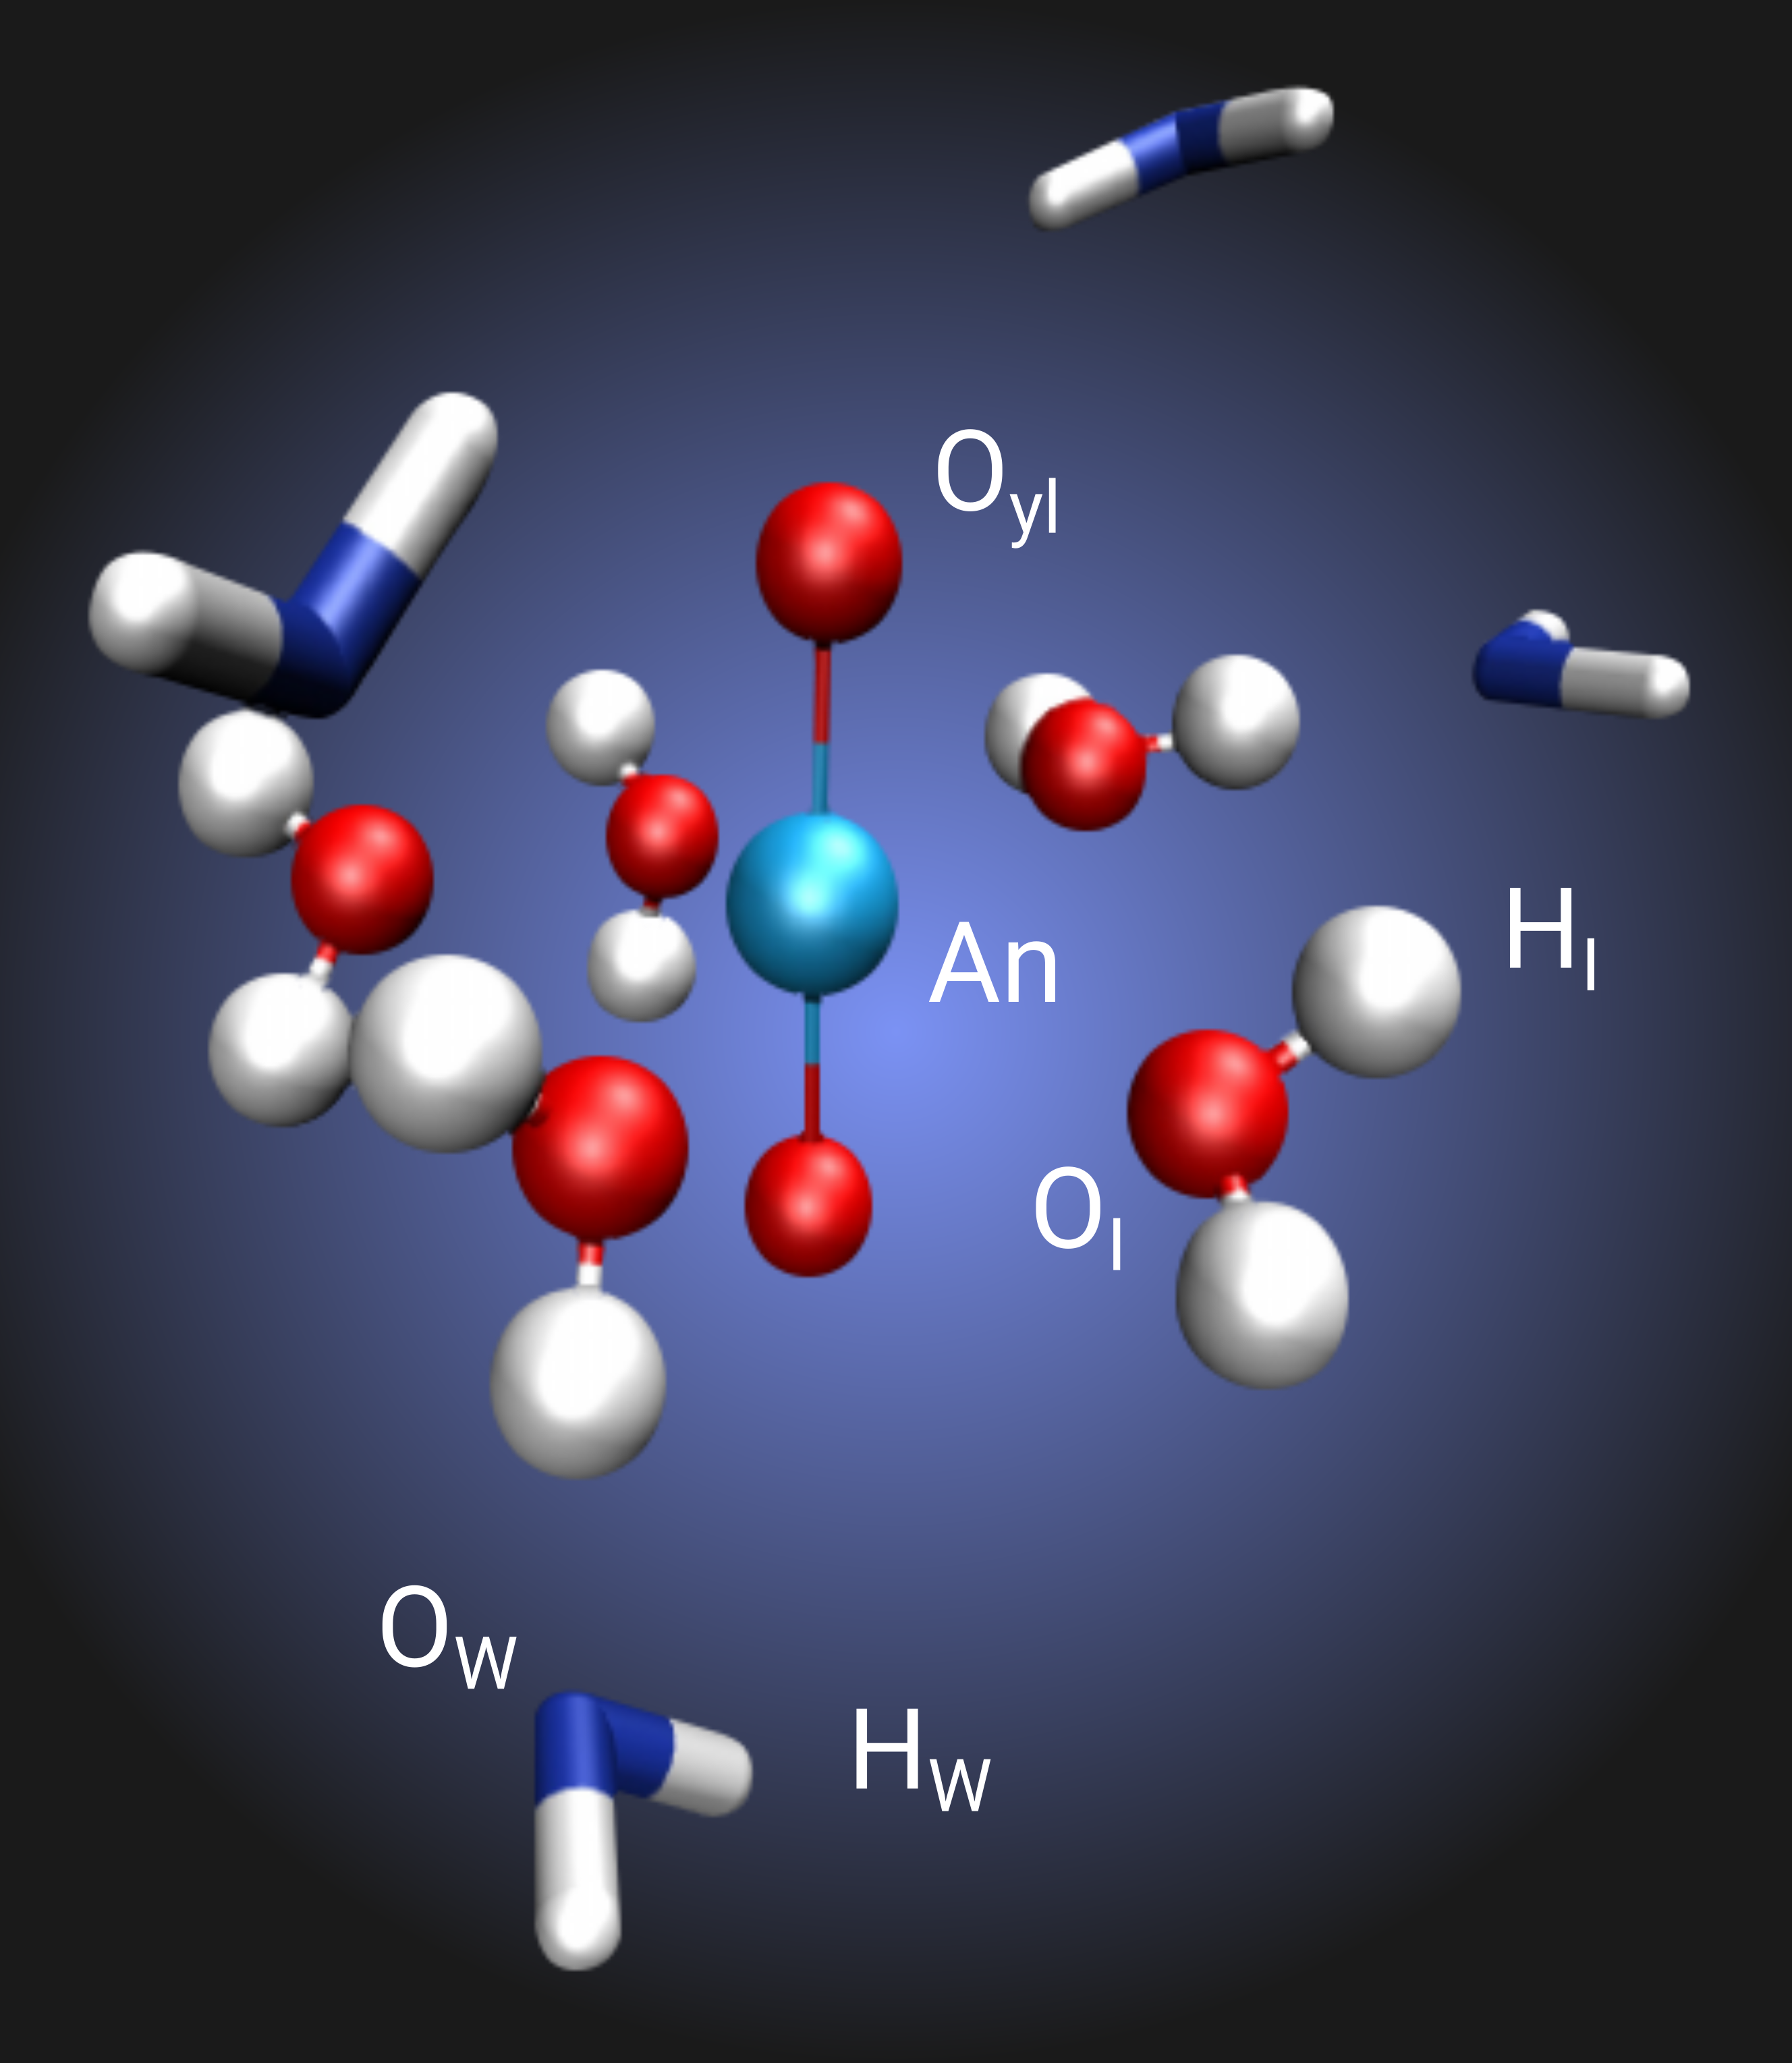
\includegraphics[width=8cm]{./images/HI_labels.png}
\caption[Hydrated ion atom types]{Image of an actinyl hydrated cation \ce{[An*(H2O)5]^{n+}} in 
water. Only some bulk water molecules are drawn for clarity. Bulk water molecules are drawn with 
the ``licorice'' representation and first-shell water molecules are represented with the ``ball and 
stick'' representation.}
\label{HI_labels}
\end{figure}

The considerations of the HI as the consistent molecular cation in solution allows us to assign 
different atom types (\ce{O_I} and 
\ce{H_I}) in first-shell water molecules than in the rest of bulk water molecules (\ce{O_W} 
and \ce{H_W}). Figure \ref{HI_labels} illustrates this. The HIM provides great flexibility to 
the 
potential 
because the bulk water molecules can 
be modeled with conventional classical force fields (TIP4P in our case) and first-shell water 
molecules can be given different 
geometries, partial charges and interaction potentials. The first-shell water molecules can now 
have 
a higher dipole than bulk water and even be charged due to partial charge transfer from the metal 
center. Assignment of these partial charges can be done with conventional partial charge 
calculation methods like CHELPG or RESP calculated on the full HI. Charge transfer and polarization 
of the first-shell and its differentiation from the bulk is a feature of great interest for 
high-charge cations since their first-shell is specially different to bulk.

This strategy of parametrization stems from considering in a more realistic way the nature of the 
ion. Unfortunately, there is a price to pay. The payment is done in terms of complexity of the 
potential. Fortunately, this increase in complexity is manageable. Two interaction potentials must 
be fit and therefore two potential energy surfaces must be scanned: the first-shell ion potential 
energy surface which governs intra-HI motion and another for the interaction of the HI with bulk 
water. In addition, to capture properly all the effects that can be accessed with this model,
the functional form of the force fields are typically complex. The functional forms used are 
a sum of $r^{-n}$ terms and an electrostatic term:
\begin{equation}
E=\sum_{i=1}^{\substack{\text{HI} \vspace{0.02cm}\\ \text{sites} }} 
\sum_{j>i}^{\substack{\text{water} \vspace{0.02cm}\\ \text{sites} } }
\left(\frac{C_{12}^{ij}}{r_{ij}^{12}}+\frac{C_{8}^{ij}}{r_{ij}^{8}}+
\frac{C_{6}^{ij}}{r_{ij}^{6}}+
\frac{C_{4}^{ij}}{r_{ij}^{4}}+
\frac{q_iq_j}{4\pi\epsilon_0 r_{ij}}\right)
\end{equation}
Because the number of coefficients is relatively high the 
potentials are more prone to over-fitting. In addition, combination rules with 
other atom types are impossible to use. This can hinder the recycling of potentials developed for 
particular systems to others, although generalizations have been 
done\cite{JACS_ESM_1999,Martinez2004,JPhysChemB_ESM_2007}. Another 
problem associated 
to the functional form is that most MD programs do not allow using this functional 
form in a simple way limiting its use to less specialized users. Nevertheless this leads to 
the development of potentials that have very high accuracy, in particular in properties 
depending on first and second hydration shells, that can reproduce subtle experimental 
properties such as EXAFS 
spectra\cite{Angew_ESM_2010,Merkling2001,JACS_ESM_2002,caralimpio2018looking,thesisNoe}.

The problem of having new atom types for first-shell water molecules is that if they leave the 
first shell and diffuse into the bulk the model becomes unphysical. Fortunately, for 
high-charge cations this is not a problem, it is a feature. Residence times of water molecules 
of most cations with charge greater than one have timescales much longer than the simulation 
time: any change in coordination or water exchange is unphysical anyway. The HIM considers the 
HI as the molecular cation in solution so the interaction between the first-shell water oxygen 
and the metal cation may be viewed as a flexible bond. Nevertheless, this interaction 
potential 
is not a harmonic function. The \ce{M-O_I} interaction goes to zero as $r \rightarrow \infty$. The 
water molecules, in principle, can leave the first shell but the barrier to do it is high 
enough 
to prevent it in the simulation timescale. If this event were to happen, the potential 
should 
be reexamined. An additional advantage of having such a flexible functional form in the \ce{M-O_I} 
interaction is that it captures anharmonicities of the bonding which an harmonic potential is 
unable of doing. 

In some cations with low charge/radius ratio, like heavy alkalines and lanthanoids, the water 
exchange 
and the changes in coordination number are frequent. The HIM can also be used to develop potentials 
for these systems but some modifications must be done. Only one type of water molecules must be 
used and in order to capture the polarization and many body effects a polarizable potential must 
be used\cite{caralimpio2018looking,thesisNoe,Angew_ESM_2010,JChemPhys_ESM_2015}. The price to pay 
for this extra flexibility of the 
potential is that the force field becomes more computationally demanding and charge transfer to the 
first shell is neglected, which should be residual anyway. This model is know as the exchangeable 
HIM. 

I will now briefly explain the historical development of the HIM across a good part of the periodic 
table. The HIM model started as solution to the problems found studying the potential energy 
surface of the \ce{Zn^{2+}} monohydrate\cite{JPhysChem_ESM_1992} therefore the first HI to be 
studied was \ce{[Zn*(H2O)6]^{2+}}.\cite{JPhysChem_ESM_1993} The HI was rigid and the parametrized 
interaction was the HI-bulk Water Interaction or $E_{HIW}$. The unprecedented  
agreement with the experimental hydration enthalpy obtained by Monte Carlo simulations  
revealed the robustness of the force field development strategy and encouraged its extension in 
a similar fashion to  \ce{[Cr*(H2O)6]^{3+}} with similar 
success\cite{JPhysChem_ESM_1996,JPhysChemB_ESM_1998}. The next 
step in the 
progression was to make the HI flexible by parametrizing its internal degrees of freedom with the 
Ion First-Shell Water potential, $E_{IW1}$. This was initially done for \ce{Cr^{3+}} but 
has become standard in the development of the HIM since.\cite{JChemPhys_ESM_1998} The great 
advantage of internal flexibility is that it allows power spectra calculation of the 
aqua ion and 
also the X-Ray Absorption Spectra which is a subtle experimental property to 
reproduce due to the high structural 
sensitivity\cite{Angew_ESM_2010,Merkling2001,JACS_ESM_2002,caralimpio2018looking,thesisNoe}. A 
variety of cations were also studied using this approach, 
\ce{Be^{2+}},\ce{Mg^{2+}},\ce{Al^{3+}},\ce{Rh^{3+}}, 
\ce{Ir^{3+}} and even \ce{Th^{4+}}.\cite{Martinez2004,JPhysChemB_ESM_2007,JACS_ESM_1999,Yang2001} 
This 
version of the HIM will be 
the one used to study actinyl pentahydrates in the thesis. The difference with previous versions is 
that the actinyl model will include an intramolecular cation interaction potential, 
$E_\text{IMC}$ which 
will define the dynamics within the actinyl unit (\ce{[AnO_2]^{2+}}). In this way we will deal with 
the fact that the cation will be molecular instead of atomic. 

Another set of cations studied using the HIM are the square planar noble metals dications, 
\ce{[M*(H2O)4]^{2+}}. The first two studied metals were \ce{[Pd*(H2O)4]^{2+}} and 
\ce{[Pt*(H2O)4]^{2+}} and its aquo-derivatives\cite{JPhysChemB_ESM_2004,Torrico2006}. A few 
years later the methodology was 
extended to study the chemotherapeutical 
cis-platin,\newline\ce{[PtCl2(NH3)2]^{2+}}.\cite{JChemTheoComp_ESM_2013,Melchior2015} The 
study of these 
compounds gave 
a picture of a single ion with two solvation environments: one equatorial that follows conventional 
solvation and a different axial solvation. This differentiated axial solvation was 
labeled the ``meso-shell'' since it is characterized by metal-ion distances in between the first 
and the second
shell, with orientations and lability resembling the second shell. This behavior 
of a single ion having two very different solvation regions will also be encountered in 
actinyls.

The last category of HIM ions are studied with a polarizable ion and water model, 
MCDHO and MCDHO2\cite{MCDHO,MCDHO2}. This allows the possibility for water exchanges in the 
first-shell and changes in coordination number. This model is known as the exchangeable HIM. The 
main advantage of this model is the ability to study cations with fast first-shell water exchange 
rates 
and varying coordination number. There have been numerous cations studied in this way: the 
alkalines, alkaline earth metals, several lanthanoids and actinoids, \ce{Sc^{3+}} and 
\ce{Tl^{+}}\cite{caralimpio2018looking,thesisNoe,Angew_ESM_2010,Caralampio2017b,Caralampio2017,
Morales2016,Yang2001}. These models allow theoretically predicting the coordination numbers in 
solution 
which is experimentally challenging in some cases like 
\ce{Sc^{3+}}.\cite{Caralampio2017b,cotton2018scandium}





\section{X-Ray Absorption Spectroscopy}\label{sec:XAS}
If a sample of thickness, $d$, and concentration, $c$, is irradiated by light-source of 
intensity, 
$I_0$, which transmits an intensity, $I$, we can characterize the absorbance of the sample by its 
absorption coefficient, $\mu$, according to the Lambert-Beer's Law:
\begin{equation}
 \mu=\frac{1}{c\cdot d}\ln{\frac{I_0}{I}}
\end{equation}
If the light source used is an X-Ray beam, the study of $\mu$ as a function of the photon 
energy is a technique known as X-Ray Absorption Spectroscopy (\gls{xas}). One of humankind's most 
important discoveries was based on XAS: Moseley's law. In 1913, Henry Moseley discovered that the 
square root of the lowest frequency line of the XAS spectrum of an atom was 
proportional to its nuclear charge. This discovery proved that an element's position in the 
periodic table is due to its nuclear charge and not its mass, consolidating Bohr's model of the 
atom as universal across the Periodic Table. 

Twenty years after Moseley's law, Kroning discovered that the XAS spectrum of condensed 
matter atoms had a fine structure that could in principle be related to the structure around 
the absorbing atom. XAS had to wait until the seventies to become the relevant 
chemical and structural characterization technique it is today. Sayers, Stern and Lytle in 
1971 discovered that through XAS one could have access to the pseudo radial 
distribution function of the absorbing atom with its neighboring atoms.\cite{sayers1971new} XAS has 
become widely 
available by the development of the 
intense synchrotron radiation sources used to measure the spectra. 

XAS is still one of the most important techniques of structural and chemical characterization 
particularly of disordered materials and metals in solution. It provides highly detailed and 
highly accurate information of the local structure around a particular atomic center and of 
its oxidation state. It has the additional advantage that it is element specific. It can be 
used in very dilute conditions ( $10^{-4}$\si{\molar} ) becoming suitable for the study of 
highly radiotoxic elements like plutonium.

When increasing the energy of the incident X-Ray beam the absorption is low until at 
a certain energy value $\mu$ suddenly increases. At this point, the X-Ray photon has 
the exact energy as the ionization energy of one of the atom's core-electron, the photon is 
absorbed 
and the atom is ionized. This absorption jump is known as absorption edge. The absorption edge is 
element-specific and the absorbing atom is typically chosen to be the metal center. In addition, 
different core 
electrons can be ionized. This generates different edges of the element which are 
labeled by the principal quantum number of the ejected photoelectron ($n=1 \rightarrow 
K$,$n=2\rightarrow L$ 
etc). 

If the absorbing atom is a monoatomic gas, increasing the energy of the 
photon beyond the edge causes the emission of the photoelectron with additional kinetic 
energy. This results in a monotonic decay of $\mu$. If the absorbing atom 
is in a condensed phase the decrease in absorption is not monotonic but 
rather presents an oscillatory fine structure. The study of this fine structure is the basis 
of chemical and structural characterization using XAS. This oscillatory behavior depends on the 
nature of the atom and the interaction of the ejected photoelecton with the electronic density of 
the nearest neighbors of the atom. The ejected photoelectron can be backscattered by the
atoms surrounding the absorber doing a round trip out of the absorber and back. The 
constructive or destructive interference of the outgoing and ongoing photoelectron wavefunctions 
increases or decreases the probability of ionization generating the oscillatory 
behavior in $\mu$. This effect is a consequence of the particle-wave duality of electrons. 

The interference pattern is a function of the kinetic energy of the electron, the distance to the 
neighbors and its thermal fluctuation, the coordination number and other spectroscopical factors. 
Modelling this interference is the 
aim of XAS interpretation. 

\begin{figure}[h!]
\centering
\includegraphics[width=9.2cm]{./images/XAS.png}
\caption[X-Ray Absorption Spectrum]{ Sr
L-edge X-Ray 
absorption spectrum in \ce{SrCO3(s)}. The data was obtained from the XAFS spectra library of 
the University of Chicago. 
\SI{7120}{\electronvolt}-\SI{7220}{\electronvolt} region corresponds to 
XANES and \SI{7220}{\electronvolt}-\SI{7790}{\electronvolt} region to EXAFS. }\label{xas}
\end{figure}

Figure \ref{xas} shows a XAS spectrum of Sr in \ce{SrCO3(s)}. The spectrum can be divided 
in 
two distinct regions:
\begin{itemize}
 \item \textbf{\gls{xanes}}: X-ray Absorption Near Edge Structure region of the spectrum. It 
extends from the absorption edge up to 100-\SI{150}{\kilo\electronvolt}. The 
photoelectron has little energy and multiple scattering processes are dominant. Quantitative 
analysis of XANES spectra is cumbersome due to multi-atom correlations and the complexity of the 
electronic problem itself. It is generally interpreted qualitatively. The position of the edge
itself is an indicator of the absorber oxidation state. Its shape is sensible to the 
symmetry of the environment and is regarded as a fingerprint of the local structure. 
\item \textbf{\gls{exafs}}: Extended 
X-ray Absorption Fine Structure region of the spectrum. It 
extends from $\sim$\SI{150}{\electronvolt} to $\sim$\SI{1000}{\electronvolt} above the 
absorption edge. Since the photoelectron has higher kinetic energy, simple backscattering paths 
dominate. This region contains most of the structural information: bond distances, coordination 
numbers and dynamic and structural disorder, that can be extracted by the use of the EXAFS 
equation. 
\end{itemize}

\begin{figure}
\centering 
\includegraphics[width=10cm]{./images/EXAFS.png}
\label{EXAFS1}
\caption[Uranyl EXAFS spectrum]{\ce{[UO2*(H2O)5]^{2+}} (blue) and \ce{[NpO2*(H2O)5]^{2+}} (orange)
L$_{\text{III}}$-edge 
k$^3$-weighted experimental EXAFS spectra.}
\label{EXAFS}
\end{figure}

\subsection{EXAFS Spectroscopy}

Above the absorption edge the absorption coefficient, $\mu$, follows the 
equation:
\begin{equation}
\mu(E)=\mu_0(E)[1+\chi(E)]
\end{equation}
Where $\mu_0(E)$ is the absorption coefficient of the gaseous monoatomic element and $\chi(E)$ is 
the 
fine structure function or EXAFS function or simply EXAFS spectrum. $\chi(E)$ contains the 
oscillatory fine structure of the spectrum resulting from the constructive and destructive 
interference of the photoelectrons backscattering paths. The EXAFS function is written with respect 
to the wavenumber of the photoelectron, $k$:
\begin{equation}
 k=\sqrt{2m_e(E-E_0)}/\hslash
\end{equation}
Where $m_e$ is the mass of the electron, $E$ the photon energy and $E_0$ the binding energy 
(or work function). Figure \ref{EXAFS} contains examples of experimental EXAFS 
spectra. The spectrum is typically weighted by $k^2$ or $k^3$ to emphasize the 
oscillations at high $k$ values.

The EXAFS equation can be written as\cite{sayers1971new}:
\begin{equation}\label{exafs}
\chi(k)=\sum_j^{\substack{\text{path} \vspace{0.02cm}\\ \text{types} 
}}\frac{N_j}{kR_j^2}\,\,S_0^2\,\,F_j(k)\,\,\eu^{\frac{-2R_j}{\lambda(k)}}\,\,\eu^{ 
-2\sigma_j^2k^2}\,\,
\text{sen}[2kR_j+\varphi_j(k)]
\end{equation}
The function is the sum of the terms of the different path types. The path types are all 
possible closed paths that go from the absorbing atom, to one or more backscattering atoms and back 
to the absorber including some that go several times through the absorber. If the path 
has only 
``two legs'', a round trip to a neighbor, it is considered a single scattering path (\gls{ss}). 
If the 
path has more than two legs, it is considered a multiple scattering path (\gls{ms}). Figure 
\ref{MS_SS} 
illustrates the kinds of paths observed.  In most cases  paths (round trips to a neighbor) 
dominate. 

\begin{figure}
\centering 
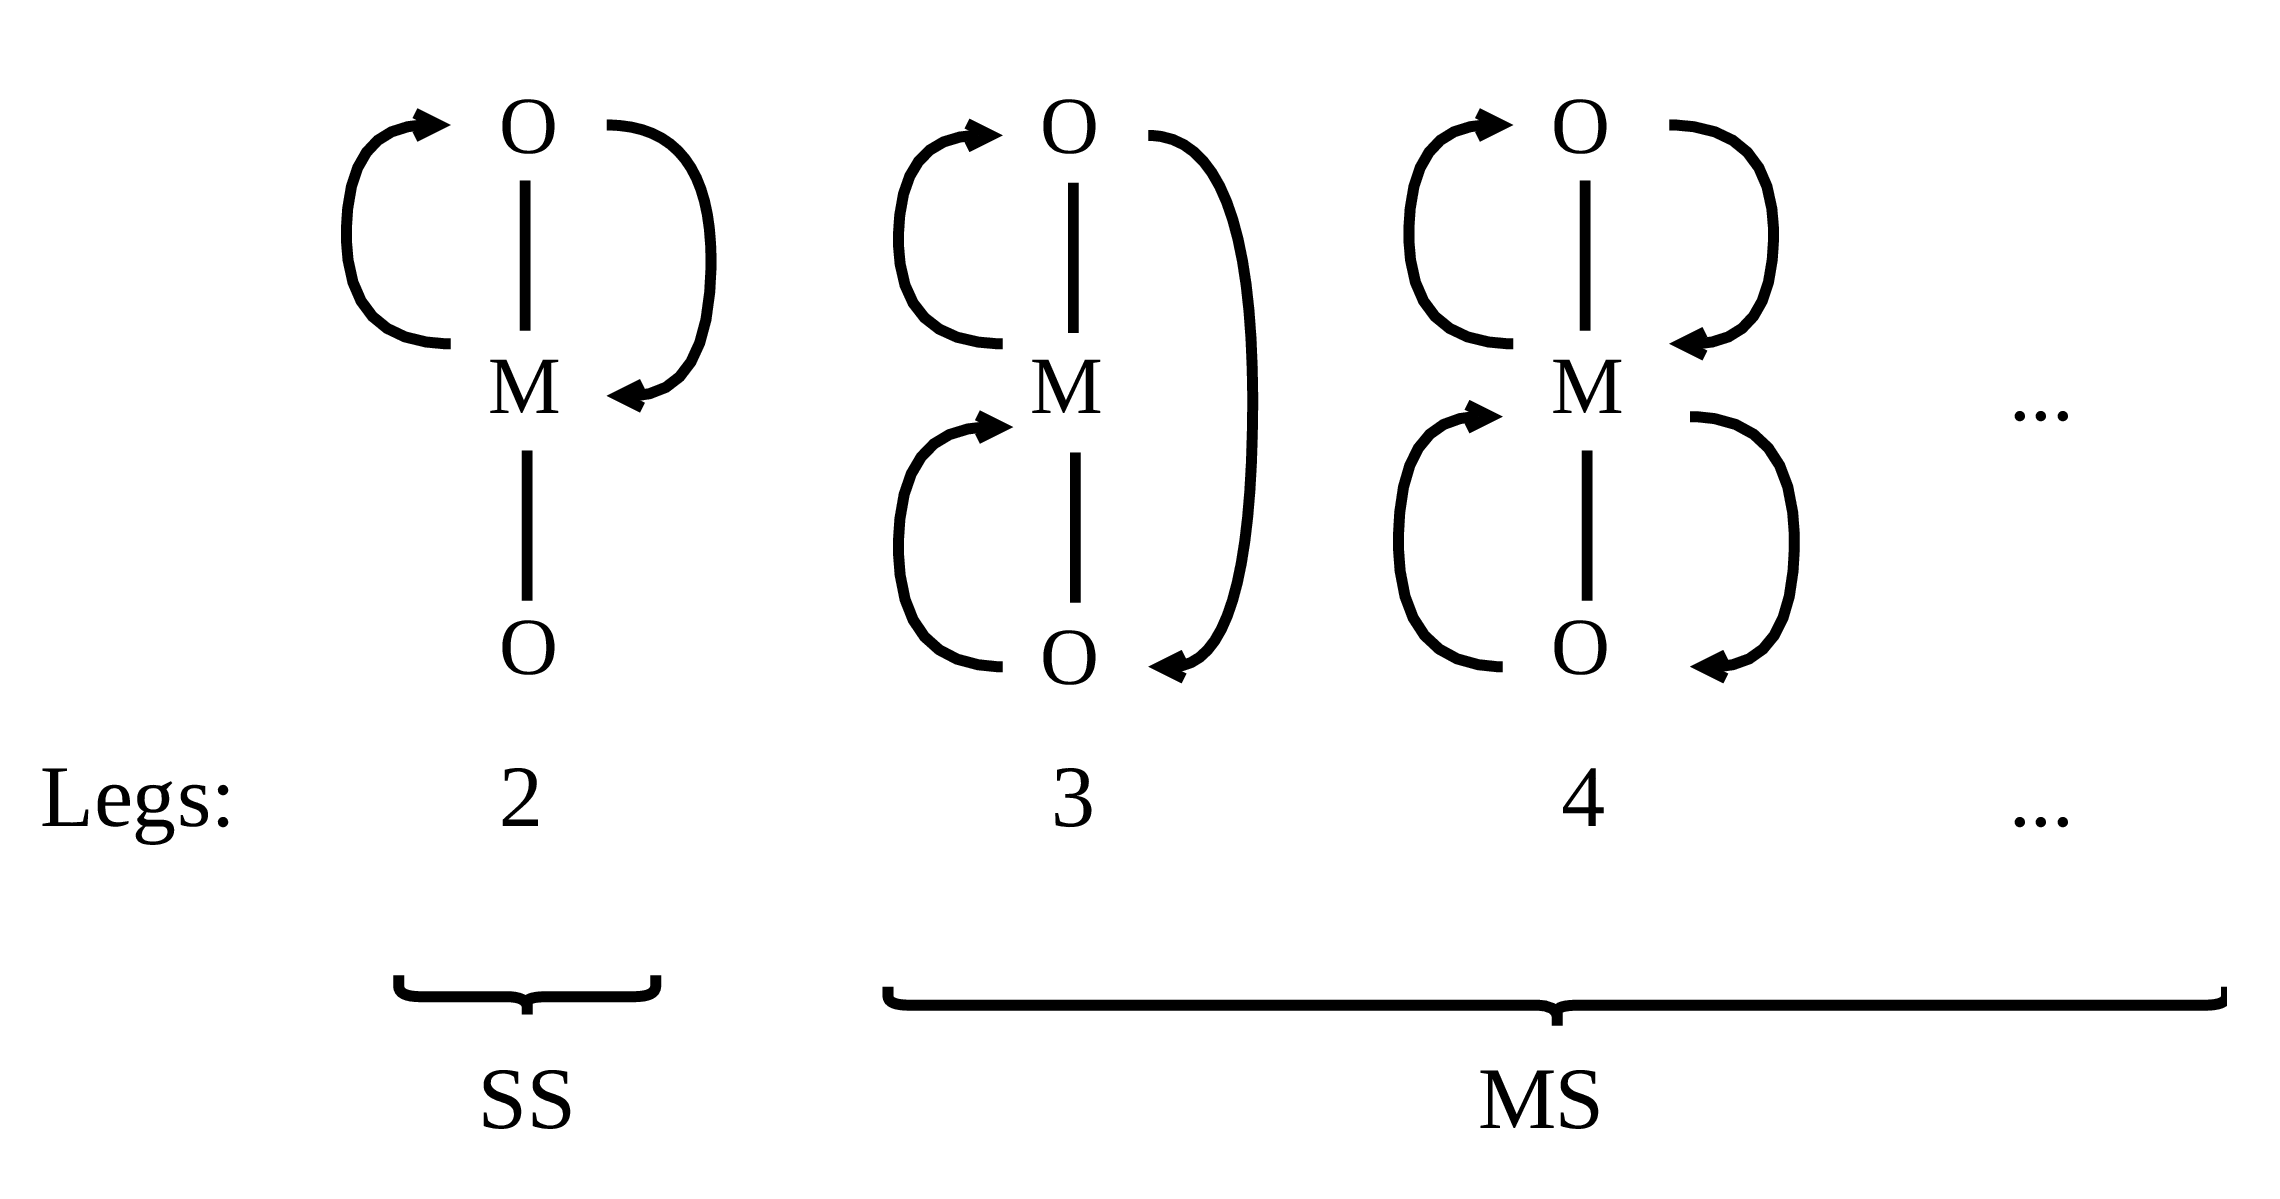
\includegraphics[width=10cm]{./images/Paths_diagram.png}
\caption[EXAFS paths illustration]{Examples of single scattering paths (\gls{ss}) and multiple scattering 
paths 
(\gls{ms}) with different number of legs. The absorber atom is M and the backscatterers are O. The 
arrows 
represent the paths the photoelectron travels.}
\label{MS_SS}
\end{figure}

The Fourier Transform of $\chi(k)$ is a pseudo-radial distribution function of the absorbing atom 
respect to its neighbor shells. It is not a true radial distribution function because multiple 
scattering paths do not depend solely on the absorber-backscatterer distance. 

First we will discuss the non-structural terms of Equation \ref{exafs} which are defined 
\textit{a priori} 
by the user or are estimated quantum-mechanically with  theoretical spectroscopy packages such 
as FEFF\cite{FEFF_PhysRevB_Rehr_2003,FEFF2_RevModPhys_Rehr_2000}.
\begin{itemize}
 \item The amplitude reduction function, $S_0^2$: It is a consequence of the 
fact that the electrons of the ionized atom experience a different potential than before the 
ionization and their wavefunction must relax to the ionized state. This factor must be included 
since only the electron and the neutral atom with a core-hole are modeled. It is typically assumed 
to have values from 0.85 to 1.0 but can also be estimated theoretically.
 \item Effective amplitude function of the path, $F_j(k)$: It has a complicated dependency on $k$ 
but it is determined by the atomic number of the backscattering atoms which serves as an
identification method for the local environment.
 \item Mean free path of the photoelectron, $\lambda(k)$: The method assumes that the wavefunction 
of 
the 
outgoing and backscattered photoelectron are coherent. This is only true during the life-time of 
the excited atom's core-hole. The method also assumes inelastic scattering. The factor $\eu^{ 
-2R_j/\lambda(k)}$ accounts for these two assumptions.
 \item Phase displacement function, $\varphi_j(k)$: Like $F_j(k)$, it has a complicated dependency 
on 
$k$ but it is determined by the atomic number of the backscattering atoms which serves as an
identification method for the local environment.
\end{itemize}
All these parameters can be nowadays calculated \textit{ab initio} by the FEFF program based on 
approximate 
relativistic quantum-mechanical self-consistent field calculations.

Now we will discuss the equation parameters that contain the structural information:
\begin{itemize}
 \item The distances to the backscattering atom, $R_j$: Actually, it is the path distance but for 
single scattering processes it coincides with the distance to the backscattering neighbor atom. 
$R_j$ control the frequency of the spectrum. Therefore, for systems with a single 
type of backscattering atoms and in the absence of significant multiple scattering contributions, 
the higher the frequency of $\chi (k)$ the longer the bondlength.
 \item The coordination number, $N_j$: Again, it is actually the degeneracy of the path but in 
single scattering processes it is equivalent to the coordination number. 
 \item The Debye-Waller Factor, $\sigma_j^2$: this parameter is the variance of the distance $R_j$ 
and measures the thermal dispersion or disorder of the path. The factor 
$\eu^{-2\sigma_j^2k^2}$ controls the envelop of the function and is responsible for the 
exponential 
decay of the fine structure. Therefore, a slowly decaying signal is associated with stiff 
structures, 
a small dispersion of path lengths and low Debye-Waller factors.
\end{itemize}

There are two ways of obtaining structural information out of an experimental EXAFS spectrum. One 
is pure experimental fitting. The spectrum is fitted to Equation \ref{exafs} with  
$\left\{R_j,N_j,\sigma_j^2\right\}$ as variables. If the spectrum has many non-equivalent 
backscattering atoms or complex features, the fitting process can be involved. In many cases, some 
of the parameters are fixed. These fixed parameters are obtained  from other experiments,
from theoretical studies or from educated guesses. This alleviates the burden of the 
high dimensionality of the problem. This fitting approach is particularly complicated in actinoids 
since there is little available experimental information for many of them so analogy with other 
actinoids is used in many cases\cite{coorchemrev_Denecke_2005}. 

In general, it is particularly difficult to fit 
with high precision the Debye-Waller factors and the coordination numbers since they are 
highly correlated. This is the reason why experimental coordination numbers obtained from EXAFS can 
have uncertainties of $\pm1$, while uncertainty in distances is much lower ($\sim\pm2\%$)

The combination of theoretical information with experimental spectra is another strategy to extract 
structural information 
from EXAFS. From the atomic positions of the absorbing atom and its nearest shells the FEFF program 
can calculate a theoretical EXAFS spectrum. If the theoretical and experimental spectra are in good 
agreement, the structural parameters of the theoretical coordinates are validated and proposed to 
characterize the system. Theoretical modelling of EXAFS is a great tool to interpret spectra, 
extract structural parameters, aid in the fitting and as a validation 
tool for newly developed theoretical models. In particular, computation of theoretical EXAFS 
spectra from statistical simulation ensembles can contribute to the interpretation of 
the experimental spectra\cite{Angew_ESM_2010,Dangelo_InorgChem_2013,spezia2017development,
ChemPhysLet_Filipponi_1994,JPhysChem_Palmer_1996,JACS_ESM_2002}. Conversely, reproducing the EXAFS 
spectrum helps to validate the quality of the simulation and the physicochemical predictions 
obtained. 

If the theoretical spectrum is calculated from a single molecular structure the Debye-Waller 
factors of the paths must be guessed since a single snapshot has no dynamic bond dispersion. 
On 
the other 
hand, if instead of a single structure we use an statistical simulation ensemble the path 
length 
dispersion is added explicitly from the statistical thermal fluctuation. The 
exponential decay term containing $\sigma_j^2$ is dropped from Equation \ref{exafs} and the 
theoretical EXAFS equation 
becomes:\cite{Merkling2001}
\begin{equation}\label{exafs-MD}
\chi(k)=\frac{1}{N_{s}}\sum_i^{N_{s}}\sum_j\frac{N_j}{kR_j^2}\,\,
S_0^2\,\,|F_j(k)|\,\,\eu^{\frac{-2R_j}{\lambda}}\text{sen}[2kR_j+\varphi_j(k)]
\end{equation}
The final spectrum is the average spectrum of the set of $N_s$ snapshots. The natural disorder 
introduced by the differences among  
the individual simulated spectra produces the exponential decay of the average function.

Both applications of the theoretical-experimental combination were done in this thesis. We used the 
theoretical EXAFS of an \ce{Am^{3+}}/\ce{[AmO2*(H2O)5]^{2+}} mixture to interpret its experimental 
EXAFS spectrum and predict the structural parameters of a pure \ce{[AmO2*(H2O)5]^{2+}} solution, a 
solution that experimentalists have been unable to produce so far.  We also used experimental EXAFS 
spectra to assess 
the quality of the actinyl force fields developed. 

More 
information of XAS spectroscopy 
can be obtained from the following 
review articles and monographs\cite{FEFF2_RevModPhys_Rehr_2000,JPhysChem_Palmer_1996,EXAFSreview, 
newville2004fundamentals,XASBook_Koningsberger_1988,AdelaCIC_v2}
. 


\section{Entropy In Molecular Dynamics Simulations}
As we have argued in Section \ref{sec:hydrophobicity}, entropy is one of the key factors in the 
hydrophobicity or 
hydrophilicity of a solute. 
Unfortunately, measuring entropic effects in simulation is a complex task. It generally involves 
either measuring the variation of free energy with temperature, $\left(\frac{\partial 
G}{\partial T}\right)_P=-S$, or by mathematically estimating how a process affects the number of 
microstates of 
a system. An example of the latter is tetrahedral entropy\cite{PNAS_Kumar_2009}.

Liquid state theory provides an additional path. The entropy of a system can be expanded as a 
sum of many-body 
correlations\cite{nettleton1958expression,baranyai1989direct}:
\begin{equation}\label{expansion}
S=S^{\left(1\right)}+S^{\left(2\right)}+S^{\left(3\right)}+\cdots
\end{equation}

This expansion has been used to study pure  
water\cite{Lazaridis1996,zielkiewicz2008two,Giuffre2010,Agarwal2011,Zhang2011} and solutions of 
simple 
solutes\cite{lazaridis1992entropy,lazaridis1994simulation,bergman1999topological,
lazaridis2000solvent,
kinoshita2006pair,liu2015order}. The use of the pair entropy expansion to calculate solvation 
entropies and 
free energies was formalized by Lazaridis in what is now commonly known as ``Inhomogeneous 
Solvation 
Theory'' 
(\gls{ist})\cite{lazaridis1998inhomogeneous}. Derivatives of this theory have been used to calculate the 
thermodynamics of structural water molecules of proteins\cite{li2012computing,Abel2008} or more 
complex solutes like amino-acids\cite{Nguyen2012,Huggins2013,Schauperl2016}

We will first assume that the system consists of a single spherically symmetric solute immersed in 
a rigid solute like the TIP4P\cite{TIP4P_JChemPhys_Jorgensen_1983} or 
SPC/E\cite{SPCE_JPhysChem_Berendsen_1987} water models.


In Equation \ref{expansion}, $S^{(1)}$  is the self correlation term, $S^{(2)}$  is the pair 
correlation term, $S^{(3)}$  
is the three-body correlation term, etc. Although the three-body term is expected to be 
significant, 
most of the information of the structure of the solution is in the pair 
term\cite{Lazaridis1996,nettleton1958expression,baranyai1989direct,wallace1987role}. 

The first order term, $S^{\left(1\right)}$, is the translational entropy of a non-interacting 
system: 
\begin{equation}
S^{\left(1\right)}=5k_\text{B}-k_\text{B}\ln 
\left(\rho_\text{s}\lambda_\text{s}^3\right)-k_\text{B}\ln\left(\rho_\text{w}\lambda_\text{w}
^3\right)
\end{equation}
where $\rho$ and $\lambda$ are the numeric density  and  the 
thermal 
wavelength of the solute (s) or the solvent (w) \cite{Lazaridis1996}.

The pair entropy term can be divided into three components:
\begin{equation}
S=S^{\left(2\right)}_\text{ss}+S^{\left(2\right)}_\text{sw}+S^{\left(2\right)}_\text{ww}
\end{equation}
The first term is zero due to the infinite dilution of the solute. The second term equals:
\begin{equation}
S^{\left(2\right)}_\text{sw}=-\frac{k_\text{B}\rho_\text{w}}{\Omega}\int 
\left[g(r,\boldsymbol{\omega})\ln\left(g(r,
\boldsymbol{\omega})\right)-g(r ,\boldsymbol{\omega})+1
\right]drd\boldsymbol{\omega}
\end{equation}
 Where $\Omega$ is the integral of the Euler angles of the solvent molecule and 
 $g(r,\boldsymbol{\omega})$ is the pair correlation function (PCF) of the atom and the solute. The 
PCF is a  function of the distance between the centers of mass of the particles and the 
orientation of the solvent, $\boldsymbol{\omega})$. An analogous expression exists for the 
solvent-solvent term. The solute-solvent PCF can be decomposed 
into\cite{Lazaridis1996}:
\begin{equation}
 g(r,\boldsymbol{\omega})=g(r)\cdot g(\boldsymbol{\omega}|r)
\end{equation}
Where $g(r)$ is the radial distribution function (\gls{rdf}) and $g(\boldsymbol{\omega}|r)$ is the 
conditional angular distribution function of the solute. As a consequence the solute-solvent 
pair 
entropy can be decomposed further into a translational component 
($S^{\left(2\right)}_\text{sw,tr}$) and an orientational 
($S^{\left(2\right)}_\text{sw,or}$)
component\cite{Lazaridis1996}:
\begin{align}
S^{\left(2\right)}_\text{sw}=&S^{\left(2\right)}_\text{sw,or}(r,\boldsymbol{\omega})+S^{
\left(2\right)}_\text{sw,tr
}(r)\\
S^{\left(2\right)}_\text{sw,or}=&-\frac{k_\text{B}\rho_\text{w}}{2\Omega}\int 
g(r)g(\boldsymbol{\omega}|r)\ln\left(g(\boldsymbol{\omega}|r)\right)drd\boldsymbol{\omega}\\
S^{\left(2\right)}_\text{sw,tr}(r)=&-2\pi k_\text{B}\rho_\text{w}\int 
\left[g(r)\ln\left(g(r)\right)-g(r)+1\right]dr
\end{align}

Recent work used the translational pair entropy as a 
fingerprint to distinguish liquid from solid local environments in metals\cite{Piaggi2017b}  and to 
use entropy as a collective variable to drive crystallization in enhanced sampling 
simulations\cite{Piaggi2017}. 

In Chapter \ref{art5}, as a first approach, we will only use $S^{\left(2\right)}_\text{sw,tr}$ 
to 
find a simple hydrophobicity and 
hydrophilicity fingerprint to characterize the atoms of a complex solute. Our work differs from 
previous uses of Equation \ref{expansion} in that we will not be interested in calculating 
thermodynamic quantities as other methods do. We will develop a simple fingerprint with a 
very simple input like the radial distribution function which will also be a good collective 
variable in enhanced sampling simulations. In addition, the ability of the fingerprint to identify 
the hydrophobicity or hydrophilicity of the hydrated actinyl atoms will be explored. 

This section has mostly been based on the following 
works\cite{lazaridis1992entropy,lazaridis1994simulation,bergman1999topological,
lazaridis2000solvent,
kinoshita2006pair,liu2015order,Lazaridis1996,zielkiewicz2008two,Giuffre2010,Agarwal2011,
Zhang2011,lazaridis1998inhomogeneous} and experience gained during my stay with
Parrinello's
group.

\section{Metadynamics}\label{sec:metadynamics}
The main limitation of phase space sampling in MD simulations is the discretization 
of the equations of motion in timesteps. The timestep for atomistically detailed 
systems is in the order of femtoseconds to describe the normal modes of atomic motion. 
Unfortunately, many of the most interesting phenomena occur in timescales of microseconds or even 
seconds. Some of these events are chemical reactions, protein folding, crystallization, phase 
changes, ligand binding etc. The long timescales are due to high kinetic barriers which 
are only surmounted by the system in the rare event of a fluctuation which accumulates enough of 
kinetic energy in the necessary degrees of freedom. For nowadays computers and, due to Moore's 
law, for the computers of tomorrow, doing enough MD steps to reach such timescales is 
impossible in the time-span of a PhD or post-doc unless you have impressive computational 
resources. 
Parallelization can lead to study bigger systems at longer timescales, 
but unfortunately time by its own nature is serial.

In order to surpass the free energy barriers special enhanced sampling MD techniques must be 
used. Many techniques have been proposed and 
detailed reviews can be found in the literature\cite{DeVivo_JMedChem_2016,Harpole2018,Abrams2014}. 
In enhanced sampling 
techniques MD simulations are carried out with some external algorithm or bias 
favoring non-Boltzmann sampling. After the sampling, post-processing techniques 
are used to obtain the Boltzmann information of the system. Enhanced sampling methods can be 
categorized in four groups\cite{Harpole2018}:
\begin{itemize}
 \item \textbf{Thermal Fluctuation Methods} 
%  They are based on giving the system a high temperature 
% to enhance fluctuations and once transitions between states occur, the system is cooled back to 
% the target temperature. The most common one is replica exchange MD (also called 
% parallel tempering) in which replica simulations are run in parallel at different temperatures above 
% and at the target temperature.\cite{Yuji1999} A metropolis criterion is used to attempt exchanging
% temperatures between the replicas periodically during the simulation. The main advantage of this 
% technique is that it requires no previous knowledge of the system. Unfortunately, it is also very 
% computationally demanding since it scales with the square root of the number of degree of freedom 
% involved. To alleviate this effect Replica Exchange Solute Tempering can be used which 
% only increases the temperature of the solute\cite{Wang2011}.
 \item \textbf{Path-Finding Methods} 
%  They are based on the knowledge of the end states and 
% finding the minimum free energy path that connects them. They do so by iterating over 
% different possible free energy paths connecting both states. Many variants exist: transition 
% interface sampling\cite{VanErp2005}, forward flux 
% sampling\cite{Allen2005}, string method with swarms of trajectories\cite{Pan2008}, 
% milestoning\cite{Bello-Rivas2015}, dynamic importance sampling\cite{Fritsch2008}. Path-finding 
% methods are computationally inexpensive since only the minimum free energy path is sampled. Their 
% drawback is that if many low free energy paths exist they will not be explored. This is 
% unlikely for processes with high energy barriers.  
 \item \textbf{Alchemical Methods} 
%  These techniques are also based on the knowledge of the 
% end-point states and are useful only if the path linking them is not of interest. A non-physical 
% path is constructed between the end-points such that the initial state slowly disappears while the 
% final appears. Then Free Energy Perturbation theory is used to calculate the free energy 
% difference\cite{Shirts2013}. Only small perturbations can be converged: ligand binding to 
% a pocket, hydration of a solute, point mutations, conversions between related species etc.
\item \textbf{Collective Variable Methods}  
% Collective variables (\gls{cv}) are functions of the 
% coordinates of the system which discriminate between the states of the system and are used to bias 
% or analyze simulations. They allow the projection of the system multidimensional behavior into a 
% small 
% set of relevant coarse grained coordinates. CV methods are based on finding appropriate 
% CVs that describe the transition and adding a bias potential on them to 
% enhance state change. For enhanced sampling simulations they should distinguish states and also 
% capture the slow normal-modes of the system that connect states. The most challenging aspect of 
% this set of methods is finding appropriate CVs in the high 
% dimensional non-linear problems tackled. Some of these techniques are: umbrella 
% sampling\cite{Torrie1977}, blue moon method\cite{Carter1989}, accelerated molecular 
% dynamics\cite{Hamelberg2004}, local elevation\cite{Huber1994}, conformational 
% flooding\cite{Loizidou2013}, adaptative force biasing\cite{Darve2008}... In this thesis we have 
% used metadynamics\cite{Laio2002} which we will review briefly.
%  \item \textbf{Hybrid methods:} There exists also many methods which combine several of the 
% previous methods for example: bias exchange metadynamics\cite{Piana2007} or parallel tempering 
% metadynamics\cite{Barducci2010}.
\end{itemize}

Metadynamics is a collective variable enhanced sampling technique in which one or several 
collective variables are biased. Collective variables (\gls{cv}) are functions of the coordinates of the 
system which discriminate between the states of the system and are used to bias 
or analyze simulations. They allow the projection of the system multidimensional behavior into a 
small  set of relevant coarse grained coordinates. CV methods like metadynamics are based on 
finding appropriate  CVs that describe the transition and adding a bias potential on them to 
enhance state change. CVs should distinguish states and also 
 capture the slow normal-modes of the system that connect states. The most challenging aspect of 
metadynamics and all CV-based methods is finding appropriate CVs in the high  dimensional 
non-linear problems tackled.

The bias 
potential 
is time-dependent and is increased in the form of Gaussians added in the regions of CV space 
that 
the system visits. The Gaussians deposited accumulate in the free energy wells the system has 
visited filling them up as if ``adding sand to fill a valley''. In the Well-Tempered version of 
metadynamics\cite{Barducci2008,Dama2014} (\gls{wtmetad}) this filling of the wells converges 
asymptotically\cite{Dama2014}. 
We shall only refer to WTMetaD which was the method used in this work. We will assume only one CV, 
$s$ is being biased for simplicity but the generalization to many CVs is straightforward.

\begin{figure}
\centering 
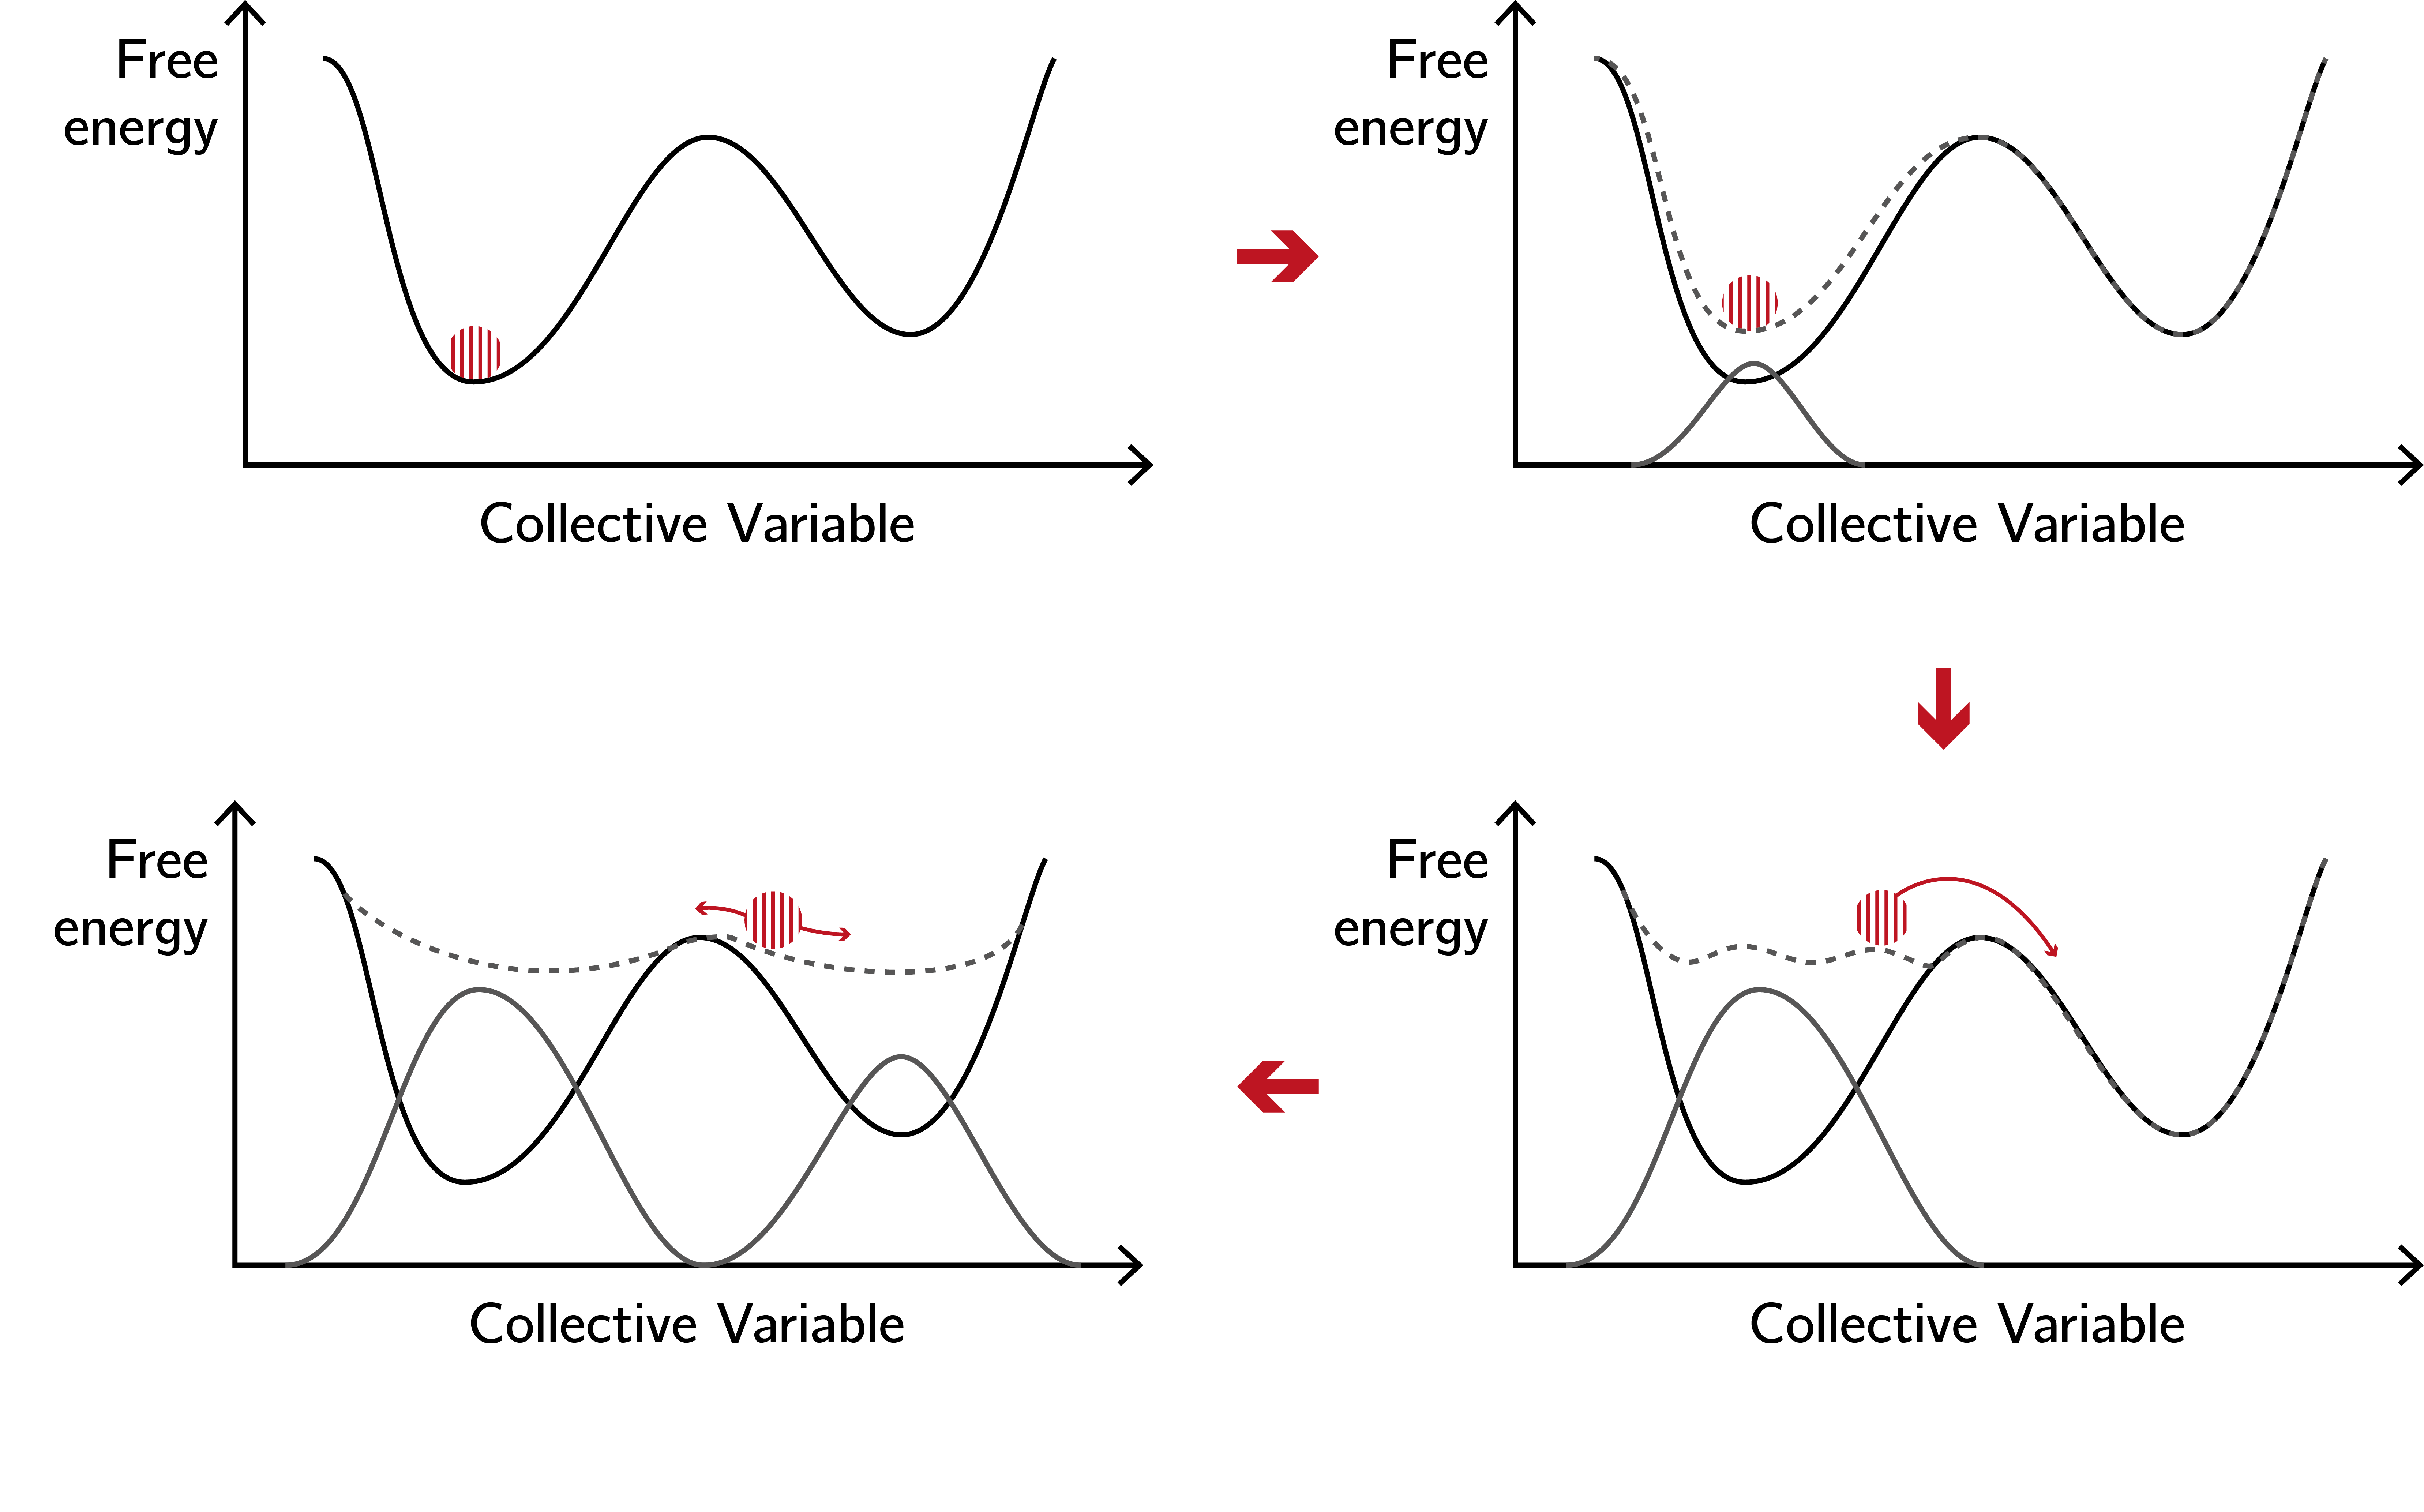
\includegraphics[width=\columnwidth]{./images/MetaD.png}
\caption[Metadynamics algorithm]{Time evolution of a system in a metadynamics simulation. The free 
energy surface of a system, $F(s)$, as a function of 
a collective variable, $s$, is represented as well as the biases (bellow the FES) and the 
CV-space position of the system (black circle). The dashed lines represent the FES that the 
biased system is experiencing due to the bias. The figure was adapted by Adriana Pérez Conesa 
based on the figure of Bussi and Branduardi.\cite{bussi2015free_v2} }
\label{MetaD_Figure}
\end{figure}

Figure \ref{MetaD_Figure} represents schematically the evolution of a system in a metadynamics 
simulation. The free energy surface of a system, $F(s)$, as a function of 
a collective variable, $s$, is represented as well as the bias (bellow the free energy surface) and 
the CV-space position of the system (striped circle). A free energy surface (\gls{fes}) is a 
projection of the free energy of the system onto a few CVs that represent its relevant states. 
The system is initially in the left free energy basin and if the barrier to jump to the right 
basin is much higher than $k_\text{B}T$, the system will only explore the left basin. In 
metadynamics 
a bias potential is added in the form of gaussians in the regions of CV-space where the system 
has been (Figure \ref{MetaD_Figure} top right) elevating the effective free energy surface of 
the system. If the right basin accumulates enough bias, the barrier is small enough for the 
system to jump to the right basin and start exploring it and filling it with bias (Figure 
\ref{MetaD_Figure} bottom right). When the right basin is also filled with bias and effective 
free energy of the system becomes flat enough, the system diffuses in CV-space going from one 
state to the other (Figure \ref{MetaD_Figure} bottom left). From the deposited bias the 
original free energy surface of the system can be calculated.

The basis of WTMetaD is the following time-dependent bias potential:
\begin{equation}\label{bias}
V(s,t)=\sum^{n}_{k=1}W
\exp{\left[-\frac{1}{\gamma-1}\beta V_{k-1}(s_k) \right]}
\eu^{\left(s-s_k\right)^2/\sigma^2}
\end{equation}
This is the bias potential added to the system hamiltonian at time $t$, where 
$n\tau<t<(n+1)\tau$. At this time it consists of $n$ Gaussians deposited which were deposited 
every 
$\tau$ steps. 

Each of the terms in the sum is a deposited gaussian ($\eu^{\left(s-s_k\right)^2/\sigma^2}$) at 
a 
position visited by system, $s_k$, with a spread $\sigma$. The initial height of the Gaussians is 
$W$ but the height decays exponentially in the regions that already have bias deposited due to the 
factor $\exp{\left[-\frac{1}{\gamma-1}\beta V_{k-1}(s_k) \right]}$. The rate of decay is controlled 
by $\gamma$ known as bias factor which is a simulation input parameter. The exponential decay of 
heights is the difference between the initial metadynamics algorithm to WTMetaD.

\begin{figure}
\centering 
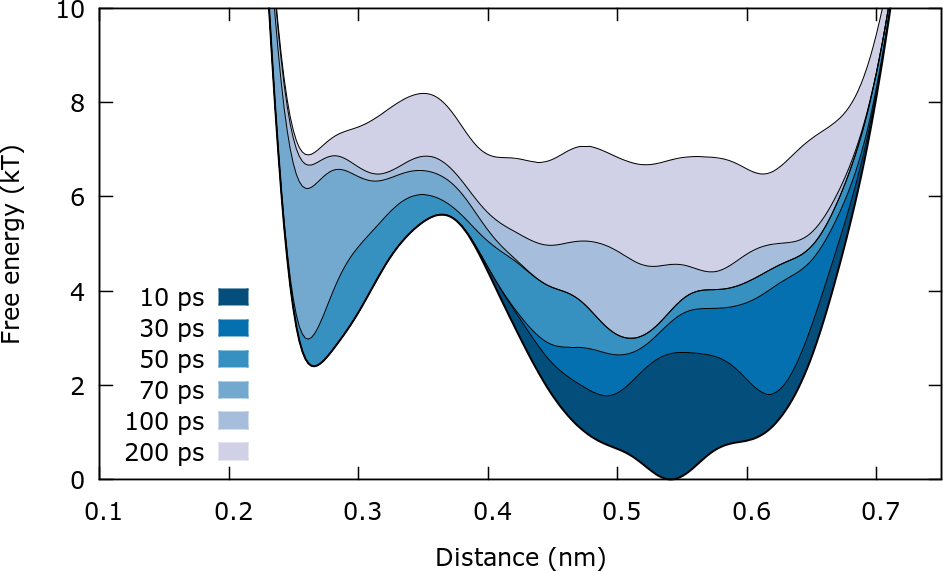
\includegraphics[width=10cm]{./images/FES_PLUMED.png}
\caption[Metadynamics free energy surface]{Free energy surface of a system as a function of 
distance 
(lower curve). Since the 
system is being simulated with metadynamics bias accumulates with time (upper curves) filling the 
free energy minima. Reproduced from the PLUMED2 manual\cite{Tribello2014}. }
\label{FES_PLUMED}
\end{figure}

 Figure \ref{FES_PLUMED} shows the free energy surface 
of a system as a function of one CV, distance,  and how the FES is filled as a function of time. 
Initially the 5$k_\text{B}T$ barrier makes the system oscillate within the right basin. After 
\SI{50}{\pico\second} so many Gaussians have been deposited in 
this region of the CV that the bias has reduced the 5$k_\text{B}T$ barrier to 2$k_\text{B}T$. 
This 
allows the system to have a fluctuation by which it jumps to the left basin. At this point 
the system starts to explore the left basin and fill it with bias. Once the two states have 
been filled with Gaussians the FES becomes somewhat flat which allows the system to cross from 
one state to the other. At this point the time-evolution of the CV becomes diffusive and if 
the heights of the Gaussians deposited are low: the simulation has converged. At convergence 
the FES experienced by the system is the unbiased FES scaled by the bias factor. 

In a converged simulation the free energy of the unbiased system as a function of the 
collective variable, 
$F(s)$, is:
\begin{equation}
F(s)=-\frac{\gamma}{\gamma-1}V(s,t)+c(t)
\end{equation}
Therefore a part from an additive constant, $c(t)$, the FES can be obtained from the simulation
deposited bias. Free energy differences between the states are calculated integrating the 
FES over their basins $A$ and $B$:
\begin{equation}
\Delta F_{A,B}=-k_\text{B}T\log\left(\frac{\int_A\eu^{-\beta F(s)}ds}{\int_B\eu^{-\beta 
F(s)}ds}\right) 
\end{equation}

WTMetaD was proposed in order to fix a problem of the original metadynamics formulation. In 
the prior formulation the height of the Gaussians deposited was constant. After the filling of 
the free energy wells of the system the bias would keep depositing forever so that the 
simulation would explore higher and higher free energy regions of CV space. It was up to the 
user to stop the simulation. WTMetaD has been proven to converge asymptotically\cite{Dama2014} 
therefore giving clear convergence conditions: the gaussian heights should be small and the CVs 
should have diffusive dynamics. 

Access to FES is not exclusive for enhanced sampling simulations. In any ergodic 
MD simulation the FES as a function of a CV, $s$, can be obtained from its 
probability distribution, $P(s)$:
\begin{equation}\label{hist2}
F(s)=-k_\text{B}T\log\left(P(s)\right)+c
\end{equation}
If the system is not ergodic, metadynamics or some other enhanced 
sampling technique must be 
used. In the case of metadynamics, Equation \ref{hist2} cannot be used directly since the 
distribution of the simulation is non-Boltzmann due to the bias. Nevertheless, the unbiased 
distribution can be estimated calculating a weighted histogram with the biased data in which the 
weights compensate biasing. This process is known as \textit{reweighting} and it can 
be done in several ways. The most accurate is the one developed recently by Tiwari and Parrinello 
which estimates the time dependent constant, $c(t)$, and in this way calculates 
exactly the bias at each step of the simulation.\cite{ReweightTiwary2015} This reweighting scheme 
uses the following 
weight for a given data point of value, $s$,  sampled at time $t$:
\begin{equation}
w(s,t)\propto\exp\left[\beta\left(V_\text{MetaD}(s,t)-c(t)+V_\text{ext}(s)\right)\right]
\end{equation}
Where $V_\text{MetaD}(s,t)$ is the WTMetaD bias, $c(t)$ the time-dependent constant and 
$V_\text{ext}(s)$ any 
additional bias added (for example only to study a certain region of the CV). Reweighting is a 
very powerful technique because it allows to project the FES on collective variables different 
than 
the ones biased in the simulation. The typical metadynamics approach is to find suitable CVs 
to converge the simulation and then reweight on to any other CV to explore the chemistry of 
the system. 

We will briefly enumerate the input parameters of a WTMetaD simulations and how they 
should be selected. In general, metadynamics is fairly robust with respect to parameter choice.
\begin{itemize}
 \item \textbf{Bias factor, $\gamma$:} It regulates the decay of the gaussian heights and 
should be chosen to be similar to the barrier size in units of $k_\text{B}T$. In the limit of 
very 
high $\gamma$ the original formulation of metadynamics is recovered. On the other hand, if $\gamma$ 
tends to 1 unbiased MD are obtained.
\item \textbf{Initial gaussian height, $W$:} It should be chosen to be 1-2$k_\text{B}T$. In 
principle 
it can be higher but it can make the equations of motion unstable due to very high biasing 
forces.
\item \textbf{Gaussian deposition frequency, $\tau$:} It should be roughly equal to the 
autocorrelation time of the CV in order for the system to ``equilibrate'' in between 
depositions. This can be estimated from unbiased simulations.
\item \textbf{Gaussian widths, $\sigma_i$:} Ideally they should be as small as possible to describe 
more accurately the underlying FES, but the smaller the width the slower the convergence. Typically 
it is set to a third or a fifth of the standard deviation of the CV in the narrowest basin in an 
unbiased simulation.
\item \textbf{Collective variables, $s_i$:} The success of metadynamics simulations is mostly 
dependent on the choice of collective variables. Ideally, only one should be used but two are 
the standard and three is also possible and necessary in some cases. Of course, the more CVs are 
biased the slower the convergence. The CVs should capture all the slow motions of the system such 
that when the bias converges there is diffusion in CV space. In many cases CV choice is cumbersome. 
Even if one useful CV has been chosen, there may be hidden orthogonal CVs that are not biased and 
prevent convergence. An example of this can be given in the context of ligand binding. Suppose the 
bias CV is only the distance between the pocket and the ligand. If the pocket is closed by the 
position of a side-chain, until there is a fluctuation and the side-chain opens the ligand will not 
bind. This will result in a decay of the gaussian heights which will barely be deposited and there 
will not be diffusion of the CV in time. To solve this, a side-chain CV should also be
biased. 
\end{itemize}

This section has mostly been based on the following 
reviews\cite{bussi2015free_v2,Valsson2016,Barducci2011}.

\bibliographystyle{achemso}
\bibliography{./library,./extrabib}
